\documentclass[german,oneside,color]{htldipl}
% Zulässige Class Options: 
%   Hauptsprache: german (default), english
%   Doppelseitig: oneside (default), twoside
%   Syntax-Highlighting: color (default), black

% die folgende Zeile einkommentieren für Arial-Ähnliche Schriftart
%\renewcommand{\familydefault}{\sfdefault}

\graphicspath{{images/}}    % Bilderverzeichnis


\usepackage[paper=a4paper,margin=3cm]{geometry}

\makeindex[title=Index]
\makeindex[name=allgemein, title=Allgemeiner Index]
\makeindex[name=name,title={Autoren Index}]
\makeindex[name=title,columns=1,title={Literatur Index}]
\indexsetup{level=\subsection*, toclevel=subsection, noclearpage}


\makeatletter
\@ifpackageloaded{biblatex_legacy}
  {\DeclareIndexNameFormat{default}{%
     \usebibmacro{index:name}{\index[name]}{#1}{#3}{#5}{#7}}}
  {\DeclareIndexNameFormat{default}{%
     \usebibmacro{index:name}{\index[name]}
       {\namepartfamily}
       {\namepartgiven}
       {\namepartprefix}
       {\namepartsuffix}}}
\makeatother

\DeclareIndexFieldFormat{indextitle}{%
  \usebibmacro{index:title}{\index[title]}{#1}}

\renewbibmacro*{bibindex}{%
  \ifbibindex
    {\indexnames{author}%
     \indexnames{editor}%
     \indexnames{translator}%
     \indexnames{commentator}%
     \indexfield{indextitle}}
    {}}

\makeatletter
\DeclareCiteCommand{\repeatfootcite}[\cbx@wrap]
  {\gdef\cbx@keys{}}
  {\xappto\cbx@keys{\thefield{entrykey},}}
  {}
  {\ifcsundef{cbx@lastin@\cbx@keys @\strfield{postnote}}
     {\csnumgdef{cbx@lastin@\cbx@keys @\strfield{postnote}}{-1}}{}%
   \ifsamepage{\value{instcount}}{\csuse{cbx@lastin@\cbx@keys @\strfield{postnote}}}
     {\footnotemark[\csuse{cbx@lastfn@\cbx@keys @\strfield{postnote}}]}
     {\xappto\cbx@cite{\noexpand\footcite%
        [\thefield{prenote}][\thefield{postnote}]{\cbx@keys}%
        \csnumgdef{cbx@lastfn@\cbx@keys @\strfield{postnote}}{\value{\@mpfn}}%
        \csnumgdef{cbx@lastin@\cbx@keys @\strfield{postnote}}{\value{instcount}}}}}

\newrobustcmd{\cbx@wrap}[1]{#1\cbx@cite\gdef\cbx@cite{}}
\def\cbx@cite{}
\makeatother

%\makeglossaries
\loadglsentries{glossary}					%beinhaltet Daten für das Glossar
\addbibresource{literatur.bib}     %beinhaltet Daten für das Literarturverzeichnis

%%%----------------------------------------------------------
\begin{document}
%%%----------------------------------------------------------
%Einstellungen an die eigene Diplomarbeit anpassen
\title{NetShare - Multi-Wan Bonding Prototyp}
\abteilung{Informatik}
%\schwerpunkt{} wenn kein Ausbildungsschwerpunkt vorhanden ist z.B. Informatik
\schwerpunkt{}
\studienort{Wiener Neustadt}
\schule{HTBLuVA Wiener Neustadt}
\schullogo{htl.jpeg}
\abgabejahr{2020/21}
\betreuerA{Dipl. Ing. Sebastian Simon}
\betreuerB{}
\betreuerC{}
\betreuerD{}
%\betreuerD{} leer lassen wenn nicht vorhanden
\schuelerA{Alexander Doubrava}
\evidenzA{5AHIF-20}
\subthemaA{Erstellen eines Multi-Wan-Bonding fähigen Proxy-Servers}
\schuelerB{Stefan Streimel}
\evidenzB{5AHIF-20}
\subthemaB{Erstellen eines Multi-Wan fähigen Windows Treiber}
\schuelerC{Martin Grafl}
\evidenzC{5AHIF-20}
\subthemaC{Alternative Lösungen, Tests, Kommunikation mit dem Treiber}
\schuelerD{Manuel Lind}
\evidenzD{5AHIF-20}
\subthemaD{Erstellen einer Windows Desktop-Anwendung zum Steuern des Treibers}
\schuelerE{}
\evidenzE{}
\subthemaE{}
%\schuelerE{} leer lassen wenn nicht vorhanden
%\evidenzE{}
%\subthemaE{}



%%%----------------------------------------------------------
\frontmatter
\maketitle
\tableofcontents
\listoffigures
%%%----------------------------------------------------------

\chapter{Vorwort}

Dies ist \textbf{Version \htldiplDate} der \latex-Dokumentenvorlage für 
die Diplomarbeiten an der HTL Wiener Neustadt, basierend auf der
Vorlage für Abschlussarbeiten an der FH Hagenberg erstellt von Dr.\ Wilhelm
Burger\footnote{\url{http://www.fh-hagenberg.at/staff/burger/diplomarbeit/}}.

Die Verwendung dieser Vorlage ist jedermann freigestellt und an
keinerlei Erwähnung gebunden. Allerdings -- wer sie als Grundlage
seiner eigenen Arbeit verwenden möchte, sollte nicht einfach
("`ung'schaut"') darauf los werken, sondern zumindest die
wichtigsten Teile des Dokuments \emph{lesen} und nach Möglichkeit
auch beherzigen. Die Erfahrung zeigt, dass dies die Qualität der
Ergebnisse deutlich zu steigern vermag.

Der Quelltext zu diesem Dokument sowie das zugehörige
\latex-Paket sind in der jeweils aktuellen Version online
verfügbar unter
%
\begin{quote}
\url{https://github.com/wschermann/Diplomarbeitsvorlage}
\end{quote}
%
Trotz großer Mühe enthält dieses Dokument zweifellos Fehler und Unzulänglichkeiten
-- Kommentare, Verbesserungsvorschläge und passende Ergänzungen
sind daher stets willkommen, am einfachsten per E-Mail direkt an mich:
\begin{center}%
\begin{tabular}{l}
\nolinkurl{w.schermann@htlwrn.ac.at} \\
Wolfgang Schermann MSc \\
HTL Wiener Neustadt -- Informatik\\
Austria
\end{tabular}
\end{center}

\noindent
Übrigens, hier im Vorwort kann man kurz auf die Entstehung  des Dokuments eingehen.
Hier ist auch der Platz für allfällige Danksagungen (\zB an den Betreuer, 
den Begutachter, die Familie, den Hund, ...), Widmungen und philosophische 
Anmerkungen. Das sollte man allerdings auch nicht übertreiben und sich auf 
einen Umfang von maximal zwei Seiten beschränken.




				%ggfs. weglassen
%Inkludiert die 4. vorgeschriebenen Seiten an Dokumentation aus dem gedruckten PDF-Formular
%Das Formular erst vor der Abgabe vollständig ausfüllen, da z.B. das Bild zur Diplomarbeit vorher nicht vorhanden sein wird
\begingroup
\makeatletter
\newpage
\@twosidefalse
\includepdf[pages=1-1,pagecommand={\chapter[Diplomarbeit Dokumentation]{}}]{pdf/Formular-printed.pdf}
\includepdf[pages=2-2,pagecommand={\thispagestyle{plain}}]{pdf/Formular-printed.pdf}
\includepdf[pages=3-3,pagecommand={\chapter[Diploma Thesis Documentation]{}}]{pdf/Formular-printed.pdf}
\includepdf[pages=4-4,pagecommand={\thispagestyle{plain}}]{pdf/Formular-printed.pdf}
\endgroup
\chapter{Kurzfassung}

An dieser Stelle steht eine Zusammenfassung der Arbeit, Umfang
max.\ 1 Seite. Im Unterschied zu anderen Kapiteln ist die
Kurzfassung (und das Abstract) üblicherweise nicht in Abschnitte
und Unterabschnitte gegliedert. 
Auch Fußnoten sind hier falsch am Platz.

Kurzfassungen werden übrigens häufig -- zusammen mit Autor und Titel
der Arbeit -- %
in Literaturdatenbanken aufgenommen. Es ist daher darauf zu
achten, dass die Information in der Kurzfassung für sich 
\emph{allein} (\dah ohne weitere Teile der Arbeit) zusammenhängend und
abgeschlossen ist. Insbesondere werden an dieser Stelle (wie \ua
auch im \emph{Titel} der Arbeit und im \emph{Abstract})
normalerweise \emph{keine Literaturverweise} verwendet! Falls man
unbedingt solche benötigt -- etwa weil die Arbeit eine
Weiterentwicklung einer bestimmten, früheren Arbeit darstellt --,
dann sind \emph{vollständige} Quellenangaben in der Kurzfassung
selbst notwendig, \zB %
[\textsc{Zobel} J.: \textit{Writing for Computer Science -- The Art of
Effective Commu\-nica\-tion}. Springer-Verlag, Singa\-pur, 1997].

Weiters sollte man daran denken, dass bei der Aufnahme in Datenbanken
Sonderzeichen oder etwa Aufzählungen mit "`Knödellisten"' in der
Regel verloren gehen. Dasselbe gilt natürlich auch für das 
\emph{Abstract}.


Inhaltlich sollte die Kurzfassung \emph{keine} Auflistung der
einzelnen Kapitel sein (dafür ist das Einleitungskapitel
vorgesehen), sondern dem Leser einen kompakten, inhaltlichen
Überblick über die gesamte Arbeit verschaffen. Der hier verwendete
Aufbau ist daher zwangsläufig anders als der in der Einleitung.
		
\chapter{Abstract}

\begin{english} 
    This diploma thesis deals with the planning and development of a multi-wan bonding prototype, called NetShare. As  Windows does not offer a free-of-charge option to use several internet connections simultaneously and to bundle their bandwidths, we decided to develop such a prototype. 
    \\\\
    For the implementation we need a multi-wan bonding capable server, driver and a Windows desktop application to control the driver. For this reason, we have dealt with the following technologies IP Routing Table, Nating, TUN-/ TAP devices, Virtual Private Networks, Winforms, and Windows drivers.
    \\\\
    In the thesis, we explain the technologies used and the approaches followed in the implementation of our multi-wan bonding prototype. Furthermore, we illustrate with the help of examples how the individual functions have been implemented. 
\end{english}
			

%%%----------------------------------------------------------
\mainmatter           %Hauptteil (ab hier arab. Seitenzahlen)
%%%----------------------------------------------------------

\chapter{Einleitung}
\label{cha:Einleitung}

\section{Projekthintergrund und Idee}
In einer Zeit der rasant voranschreitenden Digitalisierung, ist eine schnelle Internetverbindung zur Voraussetzung des täglichen Alltags geworden. Aufgrund von oft mangelhafter Infrastruktur, haben wir uns dazu entschieden einen Multi-Wan Bonding Prototyp zu entwickeln, welcher die Bündelung mehrere Internetverbindungen ermöglicht. Dadurch könnte eine schnelle und stabiler Internetanbindung erreicht werden. Es soll für den Anwender mithilfe einer simplen Desktop-Anwendung möglich sein, mehrere Internetverbindungen auszuwählen und diese gebündelt nutzen zu können.
\section{Gliederung der Diplomschrift}
\paragraph{Kapitel 2 Technologien für Multi-Wan Bonding}erläutert die verwendeten Technologien die uns bei der Implementierung des Prototypen in hinsicht auf Multi-Wan Bonding geholfen haben.
\paragraph{Kapitel 3 Technologien für Windows Desktop-Anwendungen}beschreibt die Technologien die wir zum Erstellen der Windows Desktop-Anwendung verwendet haben.
\paragraph{Kapitel 4 Verwandte Arbeiten}listet andere Lösungen im Bereich Multi-Wan Bonding auf. 
\paragraph{Kapitel 5...}
\paragraph{Kapitel 6 Multi-Wan Bonding Treiber für Windows}veranschaulicht sowohl die Herangehensweise der Implementierung, als auch die Architektur des Multi-Wan Bonding Treibers.
\paragraph{Kapitel 7 Windows Desktop-Anwendung zur Steuerung des Treibers}beschreibt die Implementierung des Designs und der Funktionalität der Desktop-Anwendung, sowie die Kommunikation mit dem Multi-Wan Bonding Treiber.
\paragraph{Kapitel 8 Funktionstests für Multi-Wan Bonding}gibt den Testaufbau und die Testergebnisse bei unseren Integrationstests wieder.
\chapter{Technologien für Multi-Wan Bonding}
\label{chap:verwendeteTechnologien}
\section{Multi-Wan Bonding}
Multi-Wan Bonding beschreibt, wie der Name schon sagt, das Bündeln einer Verbindung über mehrere WAN Zugänge. Im Normalfall handelt es sich bei WAN um das Internet.\footnote[1]{\cite[Vgl.][]{MWAN}}
\\\\
Es werden dabei verschiedene WAN-Anbindungen wie LTE, Kabel, Glasfaser, vDSL, DSL und Satellit miteinander gekoppelt, um eine ausfallsichere und schnellere Verbindung zu erhalten. Die Bandbreiten der einzelnen WAN-Anbindungen wird dabei fast summiert.$^{1}$ 

\subsection{Einsatzgebiete}
Multi-Wan Bonding kommt vorallem dann zum Einsatz, wenn eine besonders stabile Verbindung benötigt wird. Auch das Erhöhen der Bandbreite ist ein möglicher Einsatzzweck, hierfür gibt es aber bessere Lösungen.$^{1}$\footnote[2]{\cite[Vgl.][]{MWAN1}}
\\\\
Hauptsächlich wird Multi-Wan Bonding in Unternehmensnetzwerken verwendet, die eine besonders hohe Erreichbarkeit/Stabilität benötigen.\footnote[3]{\cite[Vgl.][]{MWAN2}} Oft ist es aber nicht möglich, überall eine stabile Verbindung zu erreichen. Befindet sich eine Produktionsstätte an einem abgelegenen Ort mit schlechter Infrastruktur, so ist die Gefahr einer instabilen Verbindung sehr groß. Da immer die sekundenaktuellen Informationen benötigt werden, würde dies zu einem Produktionsstop führen. Multi-Wan Bonding kann eine mögliche Lösung sein, um die Produktionsstätte hochverfügbar zu machen.$^{2}$
\\\\
Auch für Video/Audio-Streaming von Unterwegs eignet sich Multi-Wan Bonding sehr. So kann beispielsweise ein Twitch Streamer von Unterwegs mehrere SIM-Karten unterschiedlicher LTE Netzbetreiber zeitgleich verwenden, um so sicherzustellen, dass sein Stream, selbst wenn eines der Netze nicht mehr erreichbar ist nicht, unterbrochen wird.$^{2}$

\newpage
\subsection{Unterschied zu einer Normalen Verbindung}
\begin{figure}[h]
    \centering
    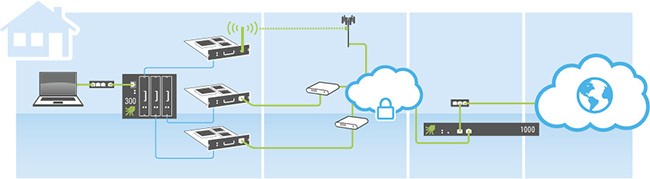
\includegraphics[width=1\textwidth]{WANB.jpg}
    \caption[Multi-WAN Bonding Konzept]{Multi-WAN Bonding Konzept}[\cite{WANB}]
\end{figure}
\noindent
Im Vergleich zu einer Normalen Verbindungsmethode handelt es sich beim Multi-Wan Bonding um eine Art von VPN Tunnel. Datenpakete laufen nicht wie gewöhnlich direkt über eine Leitung sondern werden beim Betreten des VPN Tunnels von einer Software oder Hardware Multi-Wan Lösung auf mehrere Leitungen aufgeteilt. Dies alleine ist jedoch noch nicht ganz ausreichend. Um wieder eine Verbindung zu bekommen die sich auch verwenden lässt, ist es notwendig, diese aufgeteilten Datenpakete wieder zusammen zu führen. Es gibt also einen entfernten Endpunkt, der als Proxy fungiert. Dieser Endpunkt empfängt die Datenpakete, die über die verschiedenen Verbindungen hinausgesandt wurden und setzt diese wieder zu einem Datenstrom zusammen. Damit stellt er das Ende des VPN Tunnels dar.\footnote[1]{\cite[Vgl.][]{MWAN1}}
\\\\
Es kommt dadurch selbstverständlich zu einem kleinen Datenüberhang im vergleich zu einer direkten Verbindung, da Metadaten zur Steuerung des VPN Tunnels benötigt werden. Oft werden übertragene Daten im Tunnel auch verschlüsselt.
\\\\
Da die Daten, wie bereits erwähnt, über verschiedene Verbindungen übertragen werden, die sich auch in ihrer Stabilität, Geschwindigkeit und Übertragungszeit stark unterscheiden können, muss laufend darauf geachtet werden den Datenstrom entsprechend den aktuellen Leistungs charakteristika der einzelnen Tunnel Datenströme aufzuteilen. Dies geschieht vollkommen automatisch durch die verwendete Multi-Wan Bonding Lösung und erfordert kein manuelles Eingreifen durch den Anwender.\footnote[2]{\cite[Vgl.][]{MWAN}}

\subsection{Unterschied zu Load Balancing}
Auch beim Load Balancing werden, wie beim Multi-Wan Bonding, mehrere WAN Verbindungen verwendet. Die auch im gleichen Maße vielfältig sein können.$^{1}$
\\\\
Der entscheidende Unterschied zum Multi-Wan Bonding besteht darin, dass hier das Aufteilen auf Session-Ebene stattfindet. Hier werden Sessions über den WAN Zugang laufen gelassen, der gerade am meisten Ressourcen frei hat. Beim Wan Bonding hingegen wird auf Datenpaket-Ebene aufgeteilt. Das Aufteilen auf Session-Ebene bringt Vor und Nachteile die im Folgenden dargestellt werden.$^{1}$
\newpage
\paragraph{Load-Balancing Vorteile:}\footnote[1]{\cite[Vgl.][]{MWAN3}}
\begin{enumerate}
    \item Es wird kein entfernter Endpunkt benötigt.
    \item Es gibt keinen Datenüberhang bei der Verbindung.
    \item Aufgrund eines verringerten Verarbeitungsaufwandes ist der Ping besser. 
\end{enumerate}
\paragraph{Load-Balancing Nachteile:}$^{1}$
\begin{enumerate}
    \item Bandbreite wird nicht gebündelt.
    \item Fällt eine der WAN Verbindungen aus, werden auch alle Sessions, die über diese Verbindung laufen, unterbrochen.
    \item Die Stabilität ist schlechter.
    \item Sessions haben verschiedene IP-Adressen je nach verwendeter WAN Verbindung.
\end{enumerate}


\section{IP Routing Table}
Der IP Routing Table oder Routing Table ist eine Tabelle, die alle Hosts, die an einem Netzwerk angeschlossen sind, aufbauen. Diese Tabelle wird von dem Betriebssystem verwendet um IP Pakete weiter- oder umzuleiten. Durch diese Informationen ist es außerdem möglich die Topologie des Netzwerkes, in dem sich der Host befindet, zu bestimmen.\footnote[2]{\cite[Vgl.][]{2}}
\\\\
Einträge in das Routing Table können entweder manuell, in Form von statischen Routen oder dynamisch, über Routing Protokolle erstellt werden.$^{2}$
\\\\
Ein Eintrag des Routing Table unter Linux und unter Windows hat folgende 5 Attribute: ein Netzwerkziel, eine Netzwerkmaske, ein Gateway, eine Schnittstelle und eine Metrik.$^{2}$
\\\\
Das Netzwerkziel und die Netzwerkmaske zusammen beschreiben, an welches Netzwerk ein IP Paket gerichtet sein muss, um von diesem Eintrag beeinflusst zu werden. Hier gibt es jedoch eine besondere Einstellung, wenn das Netzwerkziel als auch die Netzwerkmaske nur aus Nullen besteht. Diese Einträge werden als default Routen bezeichnet. Default Routen beeinflussen alle Pakete, bei denen folgendes \textbf{nicht} zutrifft:$^{2}$ 
\\
\begin{itemize}
    \item Es gibt keinen anderen default Routen mit einer niedrigeren Metrik.
    \item Pakete wurden vorher noch nicht von einem spezifischeren Eintrag umgeleitet.
\end{itemize}
\ \\
Das Gateway beschreibt den nächsten Hop. Genauer gesagt spiegelt es die IP-Adresse des Hosts wieder, um welches das IP-Paket umgeleitet werden muss, um in das Zielnetzwerk, oder in ein Netzwerk, das mit dem Zielnetzwerk verbunden ist, zu gelangen.$^{2}$
\\\\
Die Metrik gibt an, welcher Eintrag verwendet werden soll, wenn mehrere Einträge gleiche Werte im Netzwerkziel und in der Netzwerkmaske haben. Sie gibt bei dynamischen Routen an, wie viele Hops das IP Paket braucht, um beim Gateway anzukommen. Deswegen wird auch die kleinere Metrik bevorzugt, weil weniger Hops in der Regel weniger Latenz bedeuteten.$^{2}$
\newpage
\noindent
Die Schnittstelle gibt an, über welche Network Interface Card (NIC) das IP Paket geleitet werden muss, damit es das Gateway erreichen kann.\footnote[1]{\cite[Vgl.][]{2}}
\\\\
Eine Routing Tabelle kann wie folgt aussehen:
\\
\begin{center}
    \begin{tabular}{| c | c | c | c | c |}
        \hline
        Netzwerkziel & Netzwerkmaske & Gateway & Schnittstelle & Metrik \\
        \hline
        0.0.0.0 & 0.0.0.0 & 172.168.0.10 & 172.168.0.1 & 30 \\
        172.163.241.22 & 255.255.255.255 & 10.0.0.2 & 10.0.0.1 & 22 \\
        \hline
    \end{tabular}
\end{center}
\ \\
Bei diesem Beispiel wird ein Paket mit der IP-Adresse 172.163.241.22 an die IP-Adresse 10.0.0.2 über die Schnittstelle 10.0.0.1 weitergeleitet. Ein Paket mit IP-Adresse 30.20.10.0 wird an die IP-Adresse 172.168.0.10 über die Schnittstelle 172.168.0.1 weitergeleitet.


\section{Network Address Translation (NAT)}
NAT (Network Address Translation) dient zur Verbindung zweier getrennter Netzwerke. Im häufigsten Fall zwischen dem Internet und einem lokalen Netzwerk. Der größte Unterschied zum normalen Routing ist dabei, dass das lokale Netzwerk mit seinen IP-Adressen im Internet bzw. dem außerhalb liegenden Netzwerk nicht registriert ist. Dies hat natürlich auch zur Folge, dass IP-Adressen im lokalen Netzwerk nicht vom äußeren Netzwerk aus erreichbar sind.\footnote[2]{\cite[Vgl.][]{NAT3}}\footnote[3]{\cite[Vgl.][]{NAT1}}
\subsection{Wie funktioniert NAT?}
Wie der Name Network Address Translation (= Netzwerkadressübersetzung) schon sagt, werden dabei die nicht unbedingt global eindeutigen IP-Adressen des internen Netzwerks auf eine oder mehrere Adressen im größeren Netzwerk übersetzt. Dies geschieht gewöhnlich durch ein einzelnes Gerät z.b. einem Router. Dieser Router besitzt sowohl im lokalen unregistriertem Netzwerk eine IP-Adresse als auch im größeren Netzwerk.\footnote[4]{\cite[Vgl.][]{NAT4}}
\\\\
Erreicht den Router nun ein Datenpaket vom lokalen Netzwerk, das für eine IP-Adresse bestimmt ist, die nicht im lokalen Netzwerk liegt, so leitet er dieses Paket in das äußere Netzwerk weiter.$^{2}$ Da die IP-Adressen vom lokalen Netzwerk im äußerem Netzwerk jedoch nicht bekannt sind, hätte nun der Empfänger im äußerem Netzwerk keine Möglichkeit zu antworten. Um dieses Problem zu lösen, kommt nun der eigentliche NAT-Vorgang zum tragen. 


\newpage
\begin{figure}[h]
    \centering
    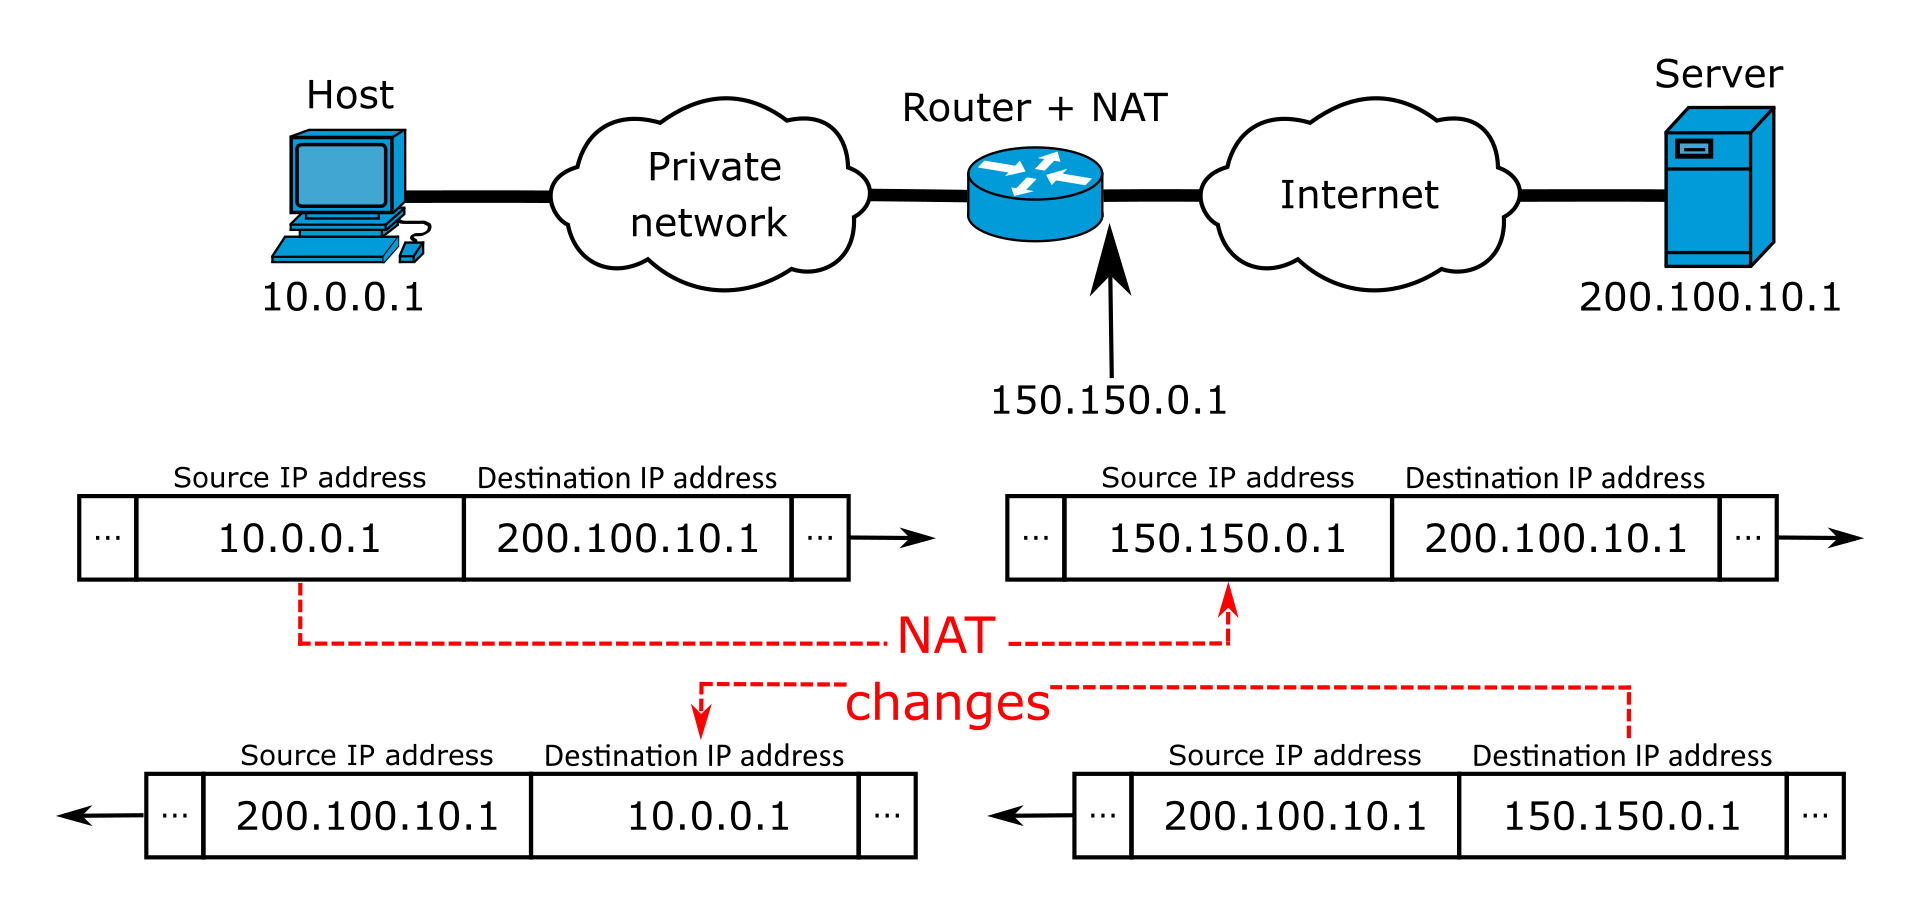
\includegraphics[width=1\textwidth]{NAT1.png}
    \caption[NAT Konzept]{NAT Konzept}[\cite{NATi1}]
\end{figure}
\noindent
Der Router der, als Mittelsmann zwischen den Netzwerken agiert, tauscht die Absenderadresse im IP-Header des lokalen Packets gegen seine eigene im äußeren Netzwerk registrierte IP-Adresse aus. Dadurch ist es nun einem Host im äußeren Netzwerk möglich, auf das Datenpaket zu antworten.\footnote[1]{\cite[Vgl.][]{NAT1}}\footnote[2]{\cite[Vgl.][]{NAT3}} 
\\\\
Kommt nun eine Antwort wieder beim Router an, wird die Ziel IP-Adresse gegen die des ursprünglichen Anfragestellers aus dem lokalen Netzwerk ausgetauscht, um im lokalen Netzwerk zugestellt werden zu können.

\newpage
\subsection{NAT Übersetzungs Tabelle}
Woher weiß nun der Router für welchen Host im lokalen Netzwerk die Antwort aus dem äußeren Netzwerk bestimmt war? 
\begin{figure}[h]
    \centering
    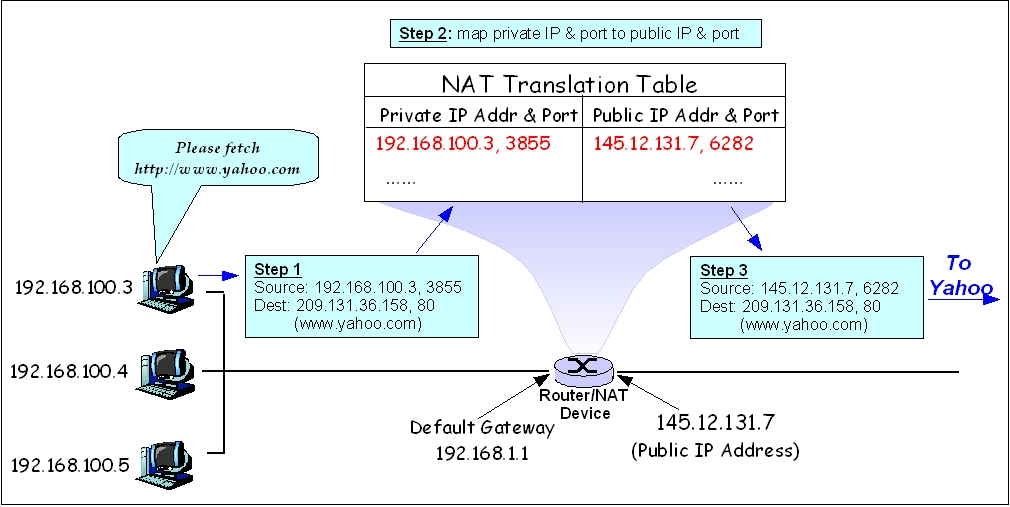
\includegraphics[width=1\textwidth]{NAT2.jpg}
    \caption[NAT Übersetzungs Tabelle]{NAT Übersetzungs Tabelle}[\cite{NATi2}]
\end{figure}
Beim Absenden der Anfrage durch den lokalen Host merkt sich der Router in der sogenannten NAT Tabelle den ursprünglichen Port und die lokale IP-Adresse, bevor er im NAT Prozess diese durch einen eigenen gewählten Port und eine eigene registrierte IP-Adresse im größerem Netz ersetzt, die er ebenfalls in die Tabelle einträgt. 
Kommt nun eine Antwort auf genau diesen äußeren Endpunkt (äußere IP-Adresse und gewählter Port vom NAT Prozess), so holt sich der Router aus der NAT Tabelle einfach die ursprüngliche Absenderadresse und den Port und setzt diese im empfangenen Antwortpaket als Zieladresse und Zielport ein.\footnote[1]{\cite[Vgl.][]{NAT5}}
\subsection{NAT und OSI Schichten}
Da der NAT Vorgang auch einen Port benötigt, ist ersichtlich, das NAT auf OSI Schicht “4 Transport” arbeitet. Das ist natürlich nicht ganz optimal, da es auf einer so hohen Schicht relativ lange dauert die Pakete umzuschreiben und weiterzuleiten. Daher werden normale Schicht drei Router vermieden und sogut es geht durch Schicht drei Switches ersetzt. NAT kann mit seinem Operationen auf Schicht vier als sehr langsam angesehen werden, im Vergleich zu den anderen häufig durchgeführten Netzwerkoperationen wie Switching und Routing.\footnote[2]{\cite[Vgl.][]{NAT6}}

\subsection{NAT und Ping (ICMP)}
Nicht alle Anwendungen verwenden zwangsläufig Ports und damit Schicht vier. Ping etwa arbeitet nur auf OSI Layer drei mit dem ICMP (Internet Control Message Protocol).\footnote[3]{\cite[Vgl.][]{NAT7}} Würde der Port einfach in der NAT Tabelle weggelassen und stattdessen nur nach Protokoll und Zieladresse zugeteilt werden, gebe es spätestens dann ein Problem, wenn zwei Hosts aus dem lokalen Netzwerk gleichzeitig den selben Host im äußerem Netzwerk anpingen. Es würde dann immer nur der Host im lokalen Netz die Antwort bekommen, der zuletzt einen Ping hinaus gesendet hat. 
\\\\
Damit dies nicht passiert, wird bei ICMP statt auf einen Port auf die ICMP Query ID geachtet.\footnote[1]{\cite[Vgl.][]{NAT1}} Diese ID wird im NAT Prozess wie der Port bei TCP, UDP Paketen behandelt. RFC 3022 schreibt dazu im Punkt 4.1 “ICMP header in ICMP Query packets must also be modified to replace the query ID and ICMP header checksum.”$^{1}$ (\cite{NAT1})

\subsection{NAT in zusammenarbeit mit Routing}
NAT alleine wird kaum eingesetzt, sondern passiert sogut wie immer im Zusammenhang mit einem Router. 
\\\\
Ob zuerst gerouted wird oder zuerst NAT angewandt hängt ganz davon ab, ob es sich um Pakete vom lokalen Netzwerk, für das äußere Netzwerk handelt oder ob es äußere Pakete sind, die in das lokale Netzwerk wollen.
Im ersten Fall, wenn Pakete aus dem lokalen Netzwerk gesendet werden, wird NAT erst kurz vor dem Verlassen des Netzwerkadapters auf das Datenpaket angewendet.\footnote[2]{\cite[Vgl.][]{SRV20}} 
\\\\
Beim zweiten Fall, wenn ein Paket von außerhalb in das lokales Netzwerk möchte, wird direkt nach dem Eingehen beim Netzwerkadapter NAT angewandt und danach erst gerouted.$^{2}$ Dies ist notwendig, da bei NAT die Zieladresse zu einer sich im lokalen Netzwerk befindenden Adresse geändert wird.\footnote[3]{\cite[Vgl.][]{NAT3}} Es darf also nicht zuvor gerouted werden, da dies mit der falschen IP-Adresse geschehen würden. Dieses Problem würde noch größer werden, wenn es mehrere lokale Netzwerke gibt.

\subsection{NAT ist eine Notlösung}
IPv4 ist schon lange veraltet und sollte schon längst durch IPv6 abgelöst werden.\footnote[4]{\cite[Vgl.][]{NAT8}} IPv4 wurde nur noch nicht abgelöst, weil ein Großteil aller Internet Anwendungen immer noch IPv4 verwenden. Da ein harter Umstieg auf IPv6 somit bedeutet, dass ein Großteil aller aktuellen Anwendungen nicht mehr funktionieren würden, kommt dies nicht in Frage. Auch heute noch werden die meisten Anwendungen für IPv4 geschrieben. Ein Grund dafür ist, dass die meisten Entwickler mit IPv4 besser vertraut sind, ein weiterer ist, dass immer noch nicht alle Internetnutzer eine IPv6-Adresse bekommen.
\\\\
Das große Problem mit IPv4 ist die Anzahl an maximal verfügbaren IP-Adressen. Es gibt einfach nicht mehr genug für die Menge an Geräten, die das Internet verwenden. 
Hier kommt nun NAT ins Spiel.$^{4}$ NAT ermöglicht es, viele unregistrierte Netzwerke zu haben, die trotzdem Zugang zum Internet besitzen. Die IP-Adressen in diesen unregistrierten Netzwerken müssen auch nicht eindeutig sein, es kann viele kleine Netzwerke geben, die dieselben IP-Adressbereiche verwenden und mittels NAT mit dem Internet verbunden sind.
\\\\
Deswegen ist es schon lange Standard geworden, dass private Internetnutzer von Ihrem Internet Service Provider (ISP) einen NAT Router bekommen. So erhält der ganze Haushalt nur eine IP-Adresse. Alle Geräte, die der Kunde mit dem Router verbindet, sind ausschließlich im LAN, haben aber durch den NAT Router nach außen ins das Internet nur die IP-Adresse des Routers. 
\\\\
Bei LTE Routern geht dies sogar noch einen Schritt weiter. Da nicht jedem Mobiltelefon eine eigene IP-Adresse gegeben werden kann, wird bei den meisten Sendemasten schon NAT angewendet.\footnote[1]{\cite[Vgl.][]{NAT9}} Wird nun einen LTE Router für den Haushalt verwendet, so kommt es schnell zur Anwendung doppelter NAT - einmal beim Sendemasten und nocheinmal im Haus. Dies sorgt für eine Reihe an Problemen, die im nächsten Thema vorgestellt werden. 

\subsection{Probleme durch NAT}
Wie bereits beschrieben wird ein Eintrag in der NAT Tabelle nur gemacht, wenn zuerst ein Datenpaket hinaus gesendet wurde. Das bedeutet, dass ein Endpoint der sich hinter einer NAT Wall befindet, nicht aus dem Internet erreichbar ist.$^{1}$ Soll also ein Server, der öffentlich erreichbar ist hinter einer NAT Wall betrieben werden, muss auf das sogenannte Port Forwarding zurückgegriffen werden.$^{1}$ Dabei wird ein Datenpaket für einen bestimmten Port immer zu einem bestimmten Host hinter der NAT Wall weitergeleitet.$^{1}$ Alleine wäre das auch noch kein allzu großes Problem, doch sobald es wie in dem LTE Fall doppeltes NAT gibt, und kein Zugriff auf eine, der NAT Router besteht, ist auch Port Forwarding nicht mehr möglich. Dies ist fast immer der Fall wenn ein LTE Router als normal Anwender verwendet wird.


\section{Virtuelles privates Netzwerk}
Ein Virtuelles privates Netzwerk kurz VPN verwendet das Internet, um Daten verschlüsselt zu übertragen. Dies wird gemacht, indem die VPN Software die Daten beim Nutzer verschlüsselt und der Server sie wieder entschlüsselt. Die Vertraulichkeit, Integrität und Authentizität der Daten wird mithilfe von Verschlüsselungstechniken gewährt. Hier hat sich Internet Protocol Security (IPsec)\footnote[2]{\cite[Vgl.][]{31}} als Standard etabliert.\footnote[3]{\cite[Vgl.][]{29}}
\\\\
VPN wird von Firmen und auch von Privatpersonen genutzt. Firmen verwenden VPN, um ihren Mitarbeitern die Möglichkeit zu geben, von außerhalb des Firmennetzwerkes auf die Daten und Geräte der Firma zuzugreifen. Die private Nutzung von VPNs besteht darin, dass Nutzer Geoblocking umgehen wollen oder ihren Netzwerkverkehr sicherer gestalten wollen. Um Geoblocking zu umgehen werden Server von den VPN Anbietern auf der ganzen Welt verfügbar gemacht. Die Nutzer verbinden sich zu einem Server, senden die Anfrage, die Sie eigentlich an eine URL senden würden an diesen. Der Server sendet die Anfrage dann an die URL und schickt die Antwort zurück zu dem Nutzer, somit wirkt es für den Webserver so als würde der Nutzer aus dem Land kommen, wo der Server steht.$^{3}$
\begin{figure}[H]
    \centering
    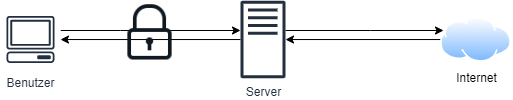
\includegraphics[width=0.8\textwidth]{VPN.png}
    \caption[Virtuelles privates Netzwerk]{Virtuelles privates Netzwerk} 
\end{figure} 


\section{Interprozesskommunikation}
Interprozesskommunikation ist der Fachbegriff für die Kommunikation zwischen verschiedenen Prozessen auf demselben Rechner. Es gibt verschiedene Arten der Interprozesskommunikation, zum einen speicherbasierte Kommunikation in Form von Shared Memory oder Dateinen und zum anderen nachrichtenbasierte Kommunikation über Message Queues, Pipes oder Sockets.\footnote[1]{\cite[Vgl.][]{30}} 


\subsection{Shared Memory}
Mehrere Prozesse greifen auf gemeinsam genutzten Speicher lesend oder schreibend zu. Der Speicher wird von einem Prozess angefordert und dann mithilfe des Betriebssystems auch in den Adressraum der anderen Prozesse eingefügt, sodass jeder Prozess darauf zugreifen kann. Shared Memory ist eine sehr simple Form der Interprozesskommunikation, die einzige Schwierigkeit ist die Synchronisation der Prozesse, also das kein Prozess gleichzeitig mit einem anderen Prozess auf den gemeinsam genutzten Speicher zugreifen kann und es somit zu keinen Race Conditions kommt.$^{1}$


\subsection{Dateien}
Mehrere Prozesse greifen auf eine Datei zu, in diese Datei werden Daten von den Prozessen geschrieben beziehungsweise gelesen. Die Prozesse dürfen wie auch auf den Shared Memory nur synchronisiert zugreifen, oftmals erfolgt dies mithilfe des Betriebssystems das den Zugriff entweder auf nur einzelne Daten der Datei oder auf die ganze Datei sperrt.$^{1}$

\subsection{Message Queue}
Daten werden an eine Nachrichtenwarteschlange gesendet, diese hat eine eindeutige Kennung, sodass die anderen Prozesse wissen aus welcher Warteschlange sie die Daten beziehen müssen. Message Queues arbeiten entweder nach dem FIFO-Prinzip (First in First out) also die Daten, die als Erstes in die Warteschlange kommen, gehen auch als Erstes wieder raus oder mithilfe von Prioritäten, sodass Prozesse die Daten mit der höchsten Priorität als Erstes aus der Warteschlange nehmen.$^{1}$ 

\newpage
\subsection{Pipes}
Die Pipe ist die erste Technik der Interprozesskommunikation, sie wurde für Unix entwickelt. Pipes kann man immer nur in eine Richtung verwenden, also ein Prozess schreibt immer und einer liest immer.  Um also Daten von einem Prozess zum anderen und wieder zurückzubefördern werden zwei unterschiedliche Pipes benötigt. Pipes sind wie auch die Massage Queues nach dem FIFO Prinzip aufgebaut. Es gibt zwei verschiedene Arten von Pipes die normalen/namenlosen Pipes und die benannten/FIFO Pipes. Der wesentliche Unterschied ist das namenlose Pipes nur von verwandten Prozessen verwendet werden können. Hingegen zu benannten Pipes die von jedem Prozess verwendet werden können, der den Namen der Pipe und die benötigten Berechtigungen hat, um eine Verbindung mit der Pipe aufzubauen.\footnote[1]{\cite[Vgl.][]{30}}

\subsection{Sockets}
Zur Kommunikation mithilfe von Sockets wird ein Server und mindestens ein Client benötigt. Der Server hat  zu jedem Client ein Socket worüber er mit diesem kommunizieren kann. Die Kommunikation erfolgt in beide Richtungen. Der Plan für Sockets war das damit verschiedene Rechner über das Netzwerk miteinander kommunizieren können. Es ist aber auch möglich damit Interprozesskommunikation zu betreiben. Indem der Server und der Client beide am selben Rechner laufen.$^{1}$
\chapter{Technologien für Windows Desktop-Anwendungen}
\label{chap:TechnologienfürWindowsDesktop-Anwendungen}

\section{GUI-Framework}

Um eine Windows-Desktop-App zu erstellen gibt es sogenannte GUI-Frameworks/-Toolkits. Diese ermöglichen dem Programmierer mit einem Designer und vorgefertigten Elementen eigene Programme im Stil von Windows zu kreieren. 
Viele Designer besitzen auch einen sogenannten Layout-Manager mit dem das Erstellen von aufwendig designten Programmen möglich wird. 
\\
\begin{figure}[H]
    \centering
    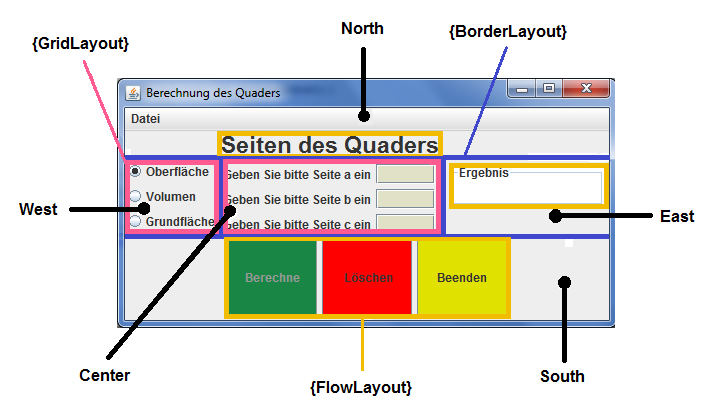
\includegraphics[width=0.8\textwidth]{LayoutTypen.png}
    \caption[Verschiedene Layout-Typen und Positionen eines Layout-Managers]{Verschiedene Layout-Typen und Positionen eines Layout-Managers}[\cite{Layout}]
\end{figure}
\noindent 
Ein weiteres Feature ist das bei GUI-Frameworks integrierte Event-Handling, welches von großem Vorteil ist, da hiermit, durch vordefinierte Ereignisse wie einem Mausklick, ein mögliches Verhalten, nach drücken eines Buttons einfach implementiert werden kann.
Nachfolgend werden nun die Frameworks WinForms und WPF vorgestellt.

\subsection{Windows Forms}

Windows Forms\footnote[1]{\cite[Vgl.][]{WindowsForms1}}, kurz WinForms ist eines der beiden bekanntesten GUI-Frameworks von Microsoft. Es gehört, genau wie das später behandelte WPF-Framework zum Microsoft 
.NET Framework.
\\
\begin{figure}[H]
    \centering
    \includegraphics[width=0.2\textwidth]{.NET-Logo.png}
    \caption[Logo von Microsoft .NET]{Logo von Microsoft .NET}[\cite{DotNet}]
\end{figure}
\noindent
WinForms wurde am 13. Februar 2002 veröffentlicht und bietet einen übersichtlichen Designer mit einer großen Auswahl an Steuerelementen sowie ein umfangreiches Event-Handling. Hiermit lässt sich mit der Programmiersprache C\# eine Desktop-Anwendung im bekannten und gewohnten Stil von Windows erstellen.\footnote[2]{\cite[Vgl.][]{WindowsForms2}}
\\
\begin{figure}[H]
    \centering
    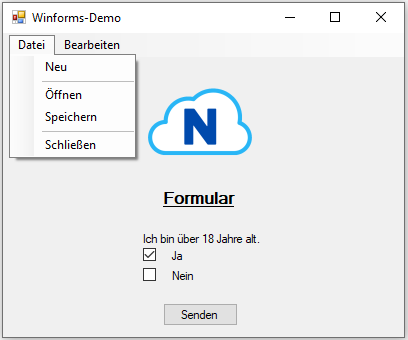
\includegraphics[width=0.5\textwidth]{Winforms-Demo.png}
    \caption[Einfache GUI mit WinForms]{Einfache GUI mit WinForms} 
\end{figure}

\subsection{Windows Presentation Foundation}
Die Windows Presentation Foundation\footnote[3]{\cite[Vgl.][]{WPF1}}, kurz WPF, ist das zweite bekannte Microsoft-Framework zur Erstellung von grafischen Benutzeroberflächen. Die auch unter dem Codenamen Avalon bekannte Klassenbibliothek erschien vier Jahre nach Windows Forms, und zwar im November 2006 im Zuge der neuen .Net-Version 3.0. Im Gegensatz zu WinForms werden in WPF Elemente wie Buttons, Menüs und weiteres üblicherweise nicht in Programmcode wie C\# definiert sondern mit der auf XML-basierenden Extensible Application Markup Language, kurz XAML.\footnote[4]{\cite[Vgl.][]{WPF2}}

\subsubsection{Extensible Markup Language}
Die sogenannte Extensible Markup Language ist eine Auszeichnungssprache, mit der man Daten, in einer hierarchisch strukturierten Form, gespeichert als Textdatei, darstellen kann. Diese wurde im Jahr 1998 vom World Wide Web Consortium veröffentlicht und hat den großen Vorteil, dass die geschriebenen Daten, sowohl von einem Mensch als auch von einem Computer, gelesen werden können. XML besteht genauso wie HTML, das vor allem für die Erstellung von Webseiten benutzt wird, aus sogenannten Tags, welche in Form von spitzen Klammern dargestellt werden. Diese Tags können ineinander verschachtelt sein sowie Parameter besitzen.\footnote[1]{\cite[Vgl.][]{XML}}
\\ \ \\
Die Auszeichnungssprache XAML ist eine eigens von Microsoft entwickelte Version von XML, welche im Zuge von und für WPF entwickelt wurde. Somit können GUI-Elemente wie in HTML einfach erstellt, beliebig angepasst und bearbeitet werden.\footnote[2]{\cite[Vgl.][]{XAML1}}
\\
\begin{figure}[H]
    \centering
    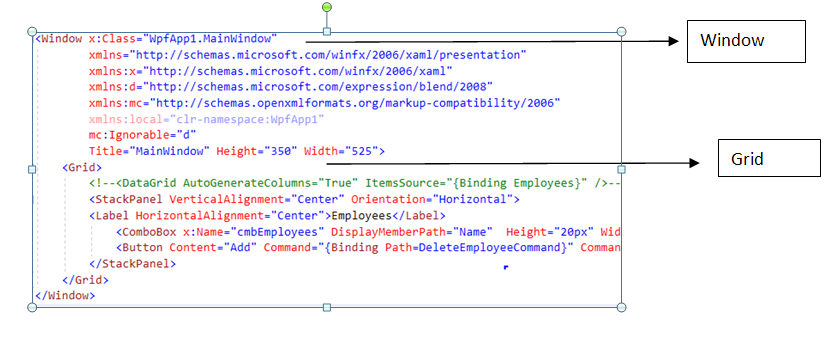
\includegraphics[width=1\textwidth]{Wpf.png}
    \caption[Erstellen einer GUI in WPF mit XAML]{Erstellen einer GUI in WPF mit XAML}[\cite{XAML2}]
\end{figure}

\subsection{Vergleich beider GUI-Frameworks}

Einer der größten Nachteile von WinForms gegenüber WPF ist, dass man sich bei der Wahl der Elemente einer GUI nur von den Standard-Windows-Bedienelementen bedienen kann. Möchte man sich also bei der Gestaltung seiner Benutzeroberfläche kreativ ausleben und zum Beispiel einen Button mit runden Ecken einbauen, so stößt man bei WinForms schnell an seine Grenzen, da es schlicht und einfach standardmäßig keinen Button mit runden Ecken in Windows gibt. Im Gegensatz dazu ist WPF nicht von den Standard-Bedienelementen von Windows abhängig und es ist so möglich, Elemente in fast allen Formen, mit fast jeder bedenklichen Funktionalität, zu kreieren. Die scheinbar grenzenlosen Möglichkeiten des GUI-Designens mit WPF können aber auch schnell zu einem Nachteil werden, denn durch die hohe Flexibilität ist es oftmals schwieriger und zeitaufwändiger ein einfaches Element zu erstellen, als es mit WinForms wäre.\footnote[3]{\cite[Vgl.][]{Vergleich}}

\subsection{Einbinden von Dynamic Link Libraries}

 Um das Problem, das man bei der Auswahl der Elemente auf die Standard-Windows-Benutzerelemente beschränkt ist zumindest größtenteils zu beheben, kann man in Visual Studio sogenannte Dynamic Link Libraries, kurz DLL, einbinden. Eine .dll-Datei ist eine Programmbibliothek, also eine Sammlung von mehreren Funktionen, welche man bei Bedarf im Hauptprogramm verwenden kann.\footnote[1]{\cite[Vgl.][]{DLL}}

\subsubsection{MetroSuite DLL}

\begin{figure}[H]
    \centering
    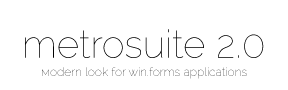
\includegraphics[width=0.5\textwidth]{MetroSuite-Logo.png}
    \caption[Logo der MetroSuite DLL]{Logo der MetroSuite DLL}[\cite{MetroSuite1}]
\end{figure}
\noindent 
Zur Umsetzung des Designs verwenden wir die MetroSuite DLL\footnote[2]{\cite[Vgl.][]{MetroSuite2}}. Mithilfe dieser ist es möglich, überarbeitete Steuerelemente oder komplett neue Komponenten in die Desktop-Anwendung einzubauen. Ein Beispiel hierfür wäre ein Button mit abgerundeten Ecken oder Animationen bei einem Mausklick auf diesen. Die MetroSuite DLL wurde von Martin Gather implementiert und steht für die nicht kommerzielle Verwendung kostenlos zur Verfügung. Aufgrunddessen, dass sich hiermit fast alle Vorstellungen umsetzen lassen, haben wir uns gegen eine kostenpflichtige Alternative und somit für MetroSuite entschieden.

\section{Grafiksoftware}

Für die visuelle Gestaltung rund um die Desktop-Anwendung benötigen wir zusätzliche Grafiksoftware, welche nachfolgend vorgestellt wird.

\subsection{Figma}

Um die Ideen rund um das Design der Desktop-Anwendung in ein sichtbares Ergebnis umzuwandeln, benutzen wir den webbasierten Vektorgrafik-Editor Figma\footnote[3]{\cite[Vgl.][]{Figma}}. Dieses Tool ermöglicht es schnell und unkompliziert Mockups zu kreieren. Dabei bietet es eine Vielzahl an vorgefertigten Formen, Schriften, Icons und weitere Elemente, die in einer Desktop-Anwendung nicht fehlen dürfen. Der große Vorteil von Figma ist, dass alle erstellten Grafiken im SVG-Format exportiert werden können. Somit können wir das Tool nicht nur für das Prototyping sondern auch zum Erstellen von Design-Elementen, welche in WinForms importiert werden können, nutzen.

\subsection{GIMP}

Neben Figma benutzen wir auch das Grafikprogramm GNU Image Manipulation Program\footnote[4]{\cite[Vgl.][]{GIMP}}, kurz GIMP. Die am 15. Februar 1996 veröffentlichte Software ist eine der bekanntesten Bildbearbeitungsprogramme, welche im Gegensatz zum Marktführer Photoshop kostenfrei zu benutzen ist. Mithilfe von GIMP kann man beispielsweise Logos oder andere Grafiken kreieren.

\section{Notification Area}
Als Notification Area werden alle rechtsbündigen Symbole bis zu dem Pfeil, der nach oben zeigt bezeichnet, wenn man auf den Pfeil klickt wird die Overflow Area geöffnet. In diesen Bereich werden standardmäßig einige Symbole verschoben. Jedes Symbol kann von der Notification Area in die Overflow Area verschoben werden dasselbe gilt auch für die andere Richtung.\footnote[1]{\cite[Vgl.][]{10}}
\begin{figure}[H]
    \centering
    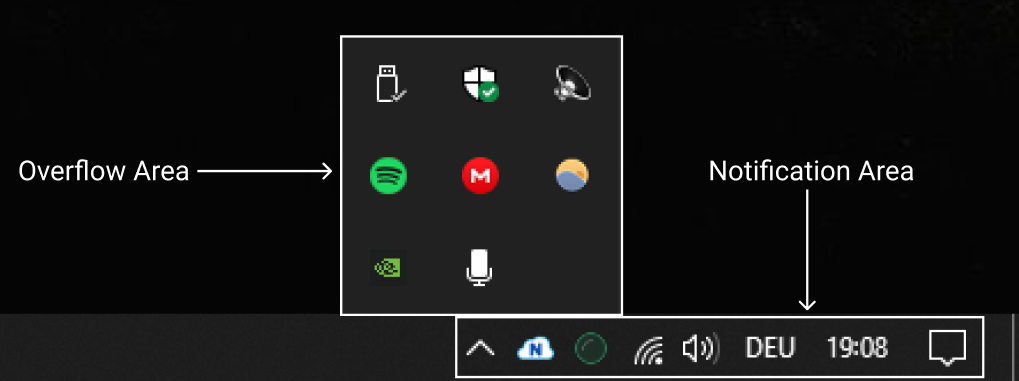
\includegraphics[width=0.8\textwidth]{NotificationArea.png}
    \caption[Notification Area]{Notification Area} 
\end{figure}
\noindent
Die Notification Area ist besser bekannt unter dem Namen Systemtray, wird aber offiziell von Windows als Notification Area bezeichnet. Der Begriff Systemtray kommt von Windows 95, weil es da eine Anwendung gibt die systray.exe heißt. Nachdem dieses Programm geschlossen wurde, sind die Symbole die in der Notification Area angezeigt wurden verschwunden. Deshalb hat man angenommen, da die Anwendung die dafür zuständig ist systray.exe heißt. Der Name des Bereichs wo die Symbole angezeigt werden Systemtray ist. Das ist aber nicht der einzige Grund der Verwirrung gewesen. Microsoft Mitarbeiter haben den Bereich als Systemtray bezeichnet und bis 2003 war auch in der Windows Dokumentation der Begriff Systemtray enthalten. Nicht nur in der Dokumentation ist Windows so ungenau, auch in den Windows 10 Einstellungen, wenn man seine Systemsprache auf Englisch hat, findet man noch den Begriff Systemtray unter Settings → Ease of Access → Narrator.\footnote[2]{\cite[Vgl.][]{15}}

\subsection{Windows Guidelines}
Dieser Bereich wurde Notification Area genannt, da der Plan war das nur Symbole gezeigt werden, die dem Benutzer hilfreiche Informationen geben entweder anhand von Benachrichtigungen oder das sich das Symbol ändert wie zum Beispiel bei der Akkustandanzeige. Ein anderer wichtiger Aspekt eines Symbols in der Notification Area ist, das die Information wichtig genug sind um den Benutzer zu stören, trotzdem aber keine sofortige  Benutzeraktion erfordert. Die Benachrichtigungen sollen ohne weiteres einfach ignoriert werden können, falls diese Benachrichtigung sofortige Benutzeraktion benötigt, wird einem vorgeschlagen, statt dieser eine Dialog Box zu benutzen. Damit wird der Benutzer dazu gezwungen etwas zu machen, wenn er seinen Computer weiter verwenden will. Es soll möglich sein die Benachrichtigungen auszuschalten. Am besten werden Benutzer nicht von ihrer Arbeit durch die Benachrichtigungen abgelenkt, sondern sehen diese erst, wenn sie schon aus einem anderen Grund den Fokus verloren haben. Viele Entwickler nutzen die Notification Area aber nicht so wie es von Windows selbst vorgeschlagen wird, sondern einfach um ihre Anwendung offenzuhalten, ohne das der normale Benutzer etwas davon weiß.\footnote[1]{\cite[Vgl.][]{17}}
\chapter{Verwandte Arbeiten}
\label{chap:VerwandteArbeiten}
Im Zuge unserer Recherche zu Multi-Wan Bonding sind wir auf verschiedene bereits existierende Hardware-/ und Software-Lösungen gestoßen, welche wir uns in diesem Kapitel genauer Ansehen werden.
Unterschied zwischen hw und sw. Hw bezahlt man einmal software abonnement hw ist standortgebunden software ist für leute die viel reisen
\section{Hardware-Lösungen}
\subsection{Multi-Wan Bonding Router}
\section{Software-Lösungen}
\subsection{Speedify}
Speedify ist eine Bereits existierende Multi-Wan Bonding Software-Lösung die das benützen von mehreren Internetverbindungen gleichzeitig möglich macht. Es ist auch eine VPN, das heißt die Daten werden verschlüsselt vom Benutzer an einen Server gesendet dieser entschlüsselt sie und sendet sie weiter ans Internet. Wenn der Server die Daten aus dem Internet wieder erhält verschlüsselt er Sie wieder und sendet die Daten an den Benutzer welcher diese dann entschlüsselt und verwenden kann.
Bei Speedify sind nur 2GB an Datenübertragung pro Monat kostenlos, wenn man mehr Datenvolumen benötigt muss man sich für ein kostenpflichtiges Abonnement entscheiden. Es gibt 3 verschiedene Abonnements bei denen sich die Anzahl an Nutzern verändert, je Nutzer kann man Speedify auf bis zu 5 Geräten gleichzeitig nutzen.
\begin{itemize}
    \item Für Einzelpersonen um 9.99 USD inkludiert 1 Benutzerkonto
    \item Für Familien um 14.95 USD mit 5 Benutzerkonten
    \item Für Firmenkunden um 9.99 USD pro Person
\end{itemize}
\  \\
Unsere Lösung ist im gegensatz zu Speedify Open Source und komplett kostenlos. Das einzige das von einem Benutzer benötigt wird, ist ein Server mit einer guten Internetanbindung, sowohl der Upload als auch der Download sind dabei wichtig.
\subsection{OpenVPN}
\chapter{Multi-Wan Bonding Proxy Server}
\label{cha:Server}

\section{Anforderungen des Multi-Wan Bonding fähigen Proxy Servers}
Unser Multi-Wan Bonding Proxy Server ist dafür verantwortlich Datenpakete des Windows Treibers zu Empfangen und zusammen zu führen und Antwortpakete aus dem Internet aufzuteilen um die an den Windows Treiber zurück zu senden. Dafür müssen Probleme gelöst werden:
\\
\begin{enumerate}
    \item Sammeln von IP Paketen von mehreren Absendeadressen für das selbe Ziel.
    \item Aufteilen von IP Paketen aus dem Internet auf mehrere Verbindungen des selben Empfängers.
    \item NAT Anwenden auf eingehende und Ausgehende IP Pakete.
\end{enumerate}
\ \\
Weiters handelt es sich bei unserem Multi-Wan Bonding Proxy Server um einen Endpunkt für die zu bündelnten Internetverbindungen. Aufgeteilte Datenpakete treffen von verschiedenen Verbindungen beim Server ein und werden wieder zu einem einzelnen Datenstrom zusammengeführt. Antworten an unseren Proxy Server werden ebenfalls entsprechend wieder aufgeteilt und an die verschiedenen WAN-Anbindungen des Nutzers gesendet. 
\\\\
Außerdem müssen gewisse Standards von Performance, Stabilität und Ressourcenanforderungen eingehalten werden. Hierbei gilt:
\\
\begin{enumerate}
    \item Maximale prozentuale CPU Auslastung von 5 {\%}, bei einer 100 Mbit/s Übertragungsrate auf einem AMD Ryzen 7 3700X
    \item Nicht mehr als 300 Megabyte RAM bedarf höchstens.
\end{enumerate}

\section{Server Infrastruktur}
\subsection{Betriebssystem}
Wir haben uns bei der Wahl des Server Betriebsystems für Linux entschieden. Um genau zu sein für Debian 8. 
Dafür gibt es einige Gründe:
\\
\begin{enumerate}
    \item Der Linux Kernel besitzt bereits Standardmäßig einen TUN/TAP Treiber was die Entwicklung des Servers um einiges vereinfacht. Bei Windows müsste man erst einen eigenen Treiber schreiben bzw. eine externe Bibliothek verwenden um einen virtuellen Netzwerkadapter zu erstellen. Dies ist unter Linux nicht notwendig.
    \item Mittels iptables ist es nur ein minimaler Aufwand NAT auf einen Netzwerkadapter anzuwenden. 
    \item Debian ist im vergleich zu Windows um einiges "leichter" damit sinken die Leistungsanforderungen an das Hostsystem erheblich. Debian benötigt Beispielsweiße keinen Desktop. Der Proxy Server selbst ist auch sehr Leistungsschonend weshalb hier schon ein älterer Raspberry PI ausreichen würde.
\end{enumerate}
\ \\
Es gibt aber viele Linux distributionen die diese Funktionalitäten haben. Warum haben wir uns also speziell für Debian 8 entschieden? Die beliebtesten Serverbetriebsysteme sind aktuell Debian, Ubuntu, CentOS und Windows ohne spezielle Reinfolge. Die entscheidung viel auf Debian weil es sich nicht nur um eine der am weitesten verbreiteten Distributionen handelt sondern auch weil es viele andere Distributionen gibt die auf Debian aufbauen. Ubuntu ist eine davon. Dies erlaubt es unserem Server auf einer vielzahl an Servern ohne hohem Aufwand zu laufen. Wir sind uns aber ziemlich sicher das es auch unter anderen Linux Distributionen keine großen Probleme geben sollte sofern man den Source-Code extra für diese kompiliert.

\subsection{Hardware}
Die Anforderungen an die Hardware sind minimal. Selbst ein schwaches Hostsystem kann unseren  Proxy Server ohne Probleme betreiben. 1GB Arbeitsspeicher ist mehr als genügend und mit 2GHz CPU Takt sollten bereits höhere Datenübertragungsraten ohne Probleme möglich sein. 
\\\\ 
Die höchste Relevanz für die Leistung unseres Proxy Servers hat die single Core Leistung des Rechners. Besonders wenn Datenraten von über 100Mbit/s das Ziel sind sollte man darauf achten.
\\\\
Die Internetanbindung ist auch von besonders hoher Relevanz. Die Summer aller mit dem Server verbundenen Nutzer kann zusammen nie eine höhere Übertragungsrate als der Hastrechner haben. 
\\\\
Festplattenspeicher wird praktisch keiner benötigt. Schon ein paar MB sind ausreichend um den Server in Betrieb zu nehmen. Vorrausgesetzt es werden keine Logfiles gespeichert.


\section{Kommunikation zwischen Server und Client}
\subsection{Der Weg eines Datenpakets von Client zu Server}
Möchte eine Anwendung etwas aus dem Internet abrufen so sendet diese Datenpakete aus. Diese Datenpakete enthalten jeweils eine Absender IP-Adresse, eine Ziel IP-Adresse, Nutzdaten und weitere Metainformationen. Diese Datenpakete müssen nun ihren weg von der Anwendung bis zum Ziel Server bestreiten. 
\\\\
Dabei werden sie, nachdem sie von der Anwendung an der Betriebsystem übergeben wurden, geroutet. Beim Routing wird für ein Datenpaket anhand der Ziel IP-Adresse ein passender Netzwerkadapter gesucht an, den das Datenpaket übergeben wird. Gibt es keine spezielle Route für diese IP-Adresse wird die sogenante Standard-Route genommen. Die Standard-Route fürt im Normalfall zu einem Router dieser Router betreibt Heutzutage erheblich mehr als nur simples Routing ins Internet. 
\\\\
Praktisch immer ist auf diesen Haushalts-Routern eine NAT Funktion aktiviert. Sollte unser Datenpaket nicht für das lokale Netzwerk bestimmt und damit wieder die Standard-Route angewandt werden muss es hier nun eine NAT Wall durchqueren. Dabei ändert sich die Absender IP-Adresse zur öffentlichen IP-Adresse des Routers bevor das Datenpaket ins Internet weitergeleitet wird. Die Ziel IP-Adresse wird später auf die öffentliche IP-Adresse des Routers Antworten.
\\\\
Um nun mehrere verschiedene Internetverbindungen zu bündeln müssen wir Datenpakete für das selbe Ziel über verschiedene Netzwerkadapter hinaussenden. Dies wird in unserem Fall von unserem Windows Treiber erledigt. Dieser leitet Datenpakete für die Standard-Route zu sich und teilt diese dann auf die physische Netzwerkadapter auf. Aufteilen alleine ist hier aber nicht genug da dann beim Zielrechner zusammengehörende Datenpakete von verschiedenen IP-Adressen ankommen würden. 
\\\\
Normale Server sind für diese Art der Kommunikation nicht ausgelegt. Besonders sehr Session behaftete Dienste sollten hier größe Probleme haben wie FTP. FTP schickt nicht mit jedem Datenpaket mit zu welchem aktuell Verbundenem FTP-Nutzer dieses Datenpaket gehört. Kommt nun ein Datenpaket von einer anderen IP-Adresse und sogar von einem anderen Port hat ein FTP-Server keine möglichkeit festzustellen zu welchem Nutzer diese Daten gehört haben. 
\\\\
Um dieses Problem zu behandeln haben wir einen Multi-Wan Bonding Proxy Server entwickeln müssen. Anstelle die Datenpakete einfach nur auf die Netzwerkadapter aufzuteilen verpackt unser Windows Treiber sie zuvor in eigenen Datenpaketen welche an unseren Proxy Server adressiert sind. Unser Server ist darauf ausgelegt von mehreren verschiedenen IP-Adressen und Ports Datenpakete zu empfanden. 
\\\\
Woher weiß unser Server welches Datenpaket zu welchem Nutzer gehört? Der Windows Treiber hat einen virtuellen Netzwerkadapter dieser virtuelle Netzwerkadapter hat eine IP-Adresse. Diese IP-Adresse können wir verwenden um verschiedene Nutzer zu unterscheiden. Aktuell haben wir aber noch keine explizite Mehrbenutzerfähigkeit eingebaut. Trotzdem ist es zumindest erforderlich das sich die IP-Adresse des virtuellen Netzwerkadapters des Nutzers im selben Subnetz befindet wir die IP-Adresse des virtuellen Netzwerkadapters des Servers. Da sonst die entpackten Datenpakete des Nutzers nicht vom virtuellen Netzwerkadapter des Servers akzeptiert werden.
\\\\
Der Server nimmt die verpackten Datenpakte, entpackt diese, wendet auf sie NAT an um sie  dann mit seiner eigenen IP-Adresse als Absender an die Ziel-Adresse zu versenden.

\subsection{Der Weg eines Datenpakets von Server zu Client}
Sendet ein Zielrechner aus dem Internet eine Antwort auf eine Anfrage unseres Proxy Servers so wird auf diese bei der Ankunft NAT angewendet. Nachdem durchschreiten der NAT Wall erhält das Datenpaket eine neue Ziel-Adresse nämlich jene die beim senden der Anfrage vom Nutzer noch unsere Absederadresse war.
\\\\
Die Absenderadresse war ursprünglich die IP-Adresse des virtuellen Netzwerkadapters unseres Windows Treibers. Anhand dieser Ziel IP-Adresse könnte der Server nun feststellen an welchen Nutzer er das Paket zurück senden muss bzw. dadurch weiters an welche der verschiedenen Eingehenden verbindungen und an welche nicht. Da Multiusersupport aber in dem Prototypen noch nicht enthalten ist wird eine Antwort aktuell einfach auf alle vorhandenen Verbindungen aufgeteilt. Die Empfänger IP-Adresse muss aber trotzdem wieder korrekt gesetzt werden da sonst der virtuelle Netzwerkadapter des Clients das Datenpaket nicht akzeptieren würde.
\\\\
Nach dem durchqueren der NAT Wall werden die Datenpakete nun einfach wieder verpackt und an die Internetadressen und Ports zurück gesendet von denen ursprünglich die Anfrage stammt.
\\\\
Nun landen die Datenpakete wieder beim Router des Nutzers bei diesem wird beim durchqueren der NAT Wall die öffentliche IP-Adresse des Nutzers wieder gegen die lokale IP-Adresse ersetzt und an das Datenpaket an den Rechner des Nutzers gerouted.
\\\\ 
Beim Rechner des Nutzers werden diese Datenpakete nun wieder vom Windows Treiber entpackt und an den virtuellen Netzwerkadapter übergeben, welcher die Datenpakte wiederum an die ursprüngliche Applikation übergibt.


\section{Architektur des Multi-Wan Bonding fähigen Proxy Servers}
\subsection{Sammeln von IP Paketen von verschiedenen Absendern}
Um IP Pakete die von unserem Windows Treiber kommen entgegennehmen zu können lauscht der Proxy Server Standardmäßig auf Port 5555 nach UDP Datagrams. 
\\\\
Jedes dieser Datagrams enthält wiederum ein IP Paket des Windows Treibers als Nutzdaten. Das IP Paket im inneren des Datagrams wird nun genommen und weiter durch den Server verarbeitet.
\\\\
Die Nutzdaten sind aber nicht die einzig Wichtigen Informationen in dem Datagram. Der Server speichert sich auch den Endpunkt von dem das Datagram gekommen ist. Dies ist Notwendig da wir davon ausgehen müssen das eine NAT Wall zwischen dem Windows Treiber und Server ist. Durch eine NAT Wall ändert sich jedoch der Absende Port und die IP Adresse. Um später also Daten auch zurück schicken zu können ist es Notwendig sich Port und IP-Adresse zu merken. Einen fixen Port können wir beim zurückschicken deswegen auch nicht nehmen.
\\\\ 
Rücksicht auf einen eventuell beschädigten Inhalt des Datagrams müssen wir auch nicht nehmen. Um die Fehlerbehandlung kümmert sich das TCP im inneren der Nutzdaten des Datagrams. Tatsächlich wäre es ein Problem TCP und nicht UDP zur übertragung zu verwenden da wir dann meistens TCP Pakete über eine TCP Verbindung senden würden. Dies würde zu einem sogenannten TCP Meltdown führen.

\subsection{Senden der gesammelten IP Pakete des Windows Treibers}
Die Nutzdaten der gesammelten Datagrams sind selbst wieder IP Pakete. Diese nehmen wir nun und übergeben als byte Arrays an den virtuellen Netzwerkadapter. Da Datenpakete betreten den virtuellen Netzwerkadapter hierbei von der selben Seite wie es bei einem physischen Netzwerkadapter die Bits und Bytes über das Patch Kabel würden.
\\\\  
Danach wird das Datenpaket gerouted. In den meisten Fällen wird es wohl ein Paket für das Internet sein es kann aber auch ein Paket für die IP-Adresse den virtuellen Netzwerkadapters des Servers sein oder für die öffentliche IP-Adresse des Servers. Sollte an dem Server noch ein weiteres Netzwerk hängen so kann das Paket auch für dieses sein. Ist es jedoch für das Internet bestimmt wird die Standard Route gewählt welche zu dem Netzwerkadapter ins Internet führt. 
\\\\
Nachdem das Paket nun gerouted wurde kommt es hier vor dem versenden ins Internet noch zur Anwendung von NAT. Der Grund dafür ist das die IP-Adresse des Servers nun vom Server selbst als auch von den Nutzern des Proxy Servers verwendet wird. Wärend diesem NAT Prozess wird die Absender IP-Adresse gegen die öffentliche IP-Adresse des Servers getauscht. Danach verlässt das Datenpaket unseren Server ins Internet.

\subsection{Entgegennehmen von Antwort Paketen aus dem Internet}
Antworten aus dem Internet werden direkt nach dem eintreffen beim Server wieder durch die NAT Wall gezogen. Dabei wird die Ziel IP-Adresse, welche bis zu diesem Punkt die öffentliche IP-Adresse des Servers war, gegen die lokale IP-Adresse des virtuellen Netzwerkadapters des Windows Treibers eingetauscht.
\\\\ 
Nun wird das Datenpaket gerouted. Da das routing Ziel die IP-Adresse des Windows Treiber seinen virtuellen Netzwerkadapter ist wird das Datenpaket an den virtuellen Netzwerkadapter des Servers übergeben. Dies geschied da sich der virtuelle Netzwerkadapter des Servers und des Windows Treibers im selben subnetz befinden müssen.  
\\\\
Nach der entgegenname durch den virtuellen Netzwerkadapter erhalten wir das IP Paket als byte array welches wir nun wieder an den Windows Treiber senden müssen.

\subsection{Senden von Antwort Paketen an den Windows Treiber}
Jene Datenpakete welche wir als Byte Arrays aus dem virtuellen Netzwerkadapter gezogen haben senden wir über die ganz normale UDP Socket API unter Linux an den Windows Treiber. 
\\\\
Dabei erstellen wird wieder ein Datagram und verwenden als Nutzdaten das IP Paket welches wir als byte array vorliegen haben. Als Zieladresse und Ziel Port verwenden wir einen der Endpunkte welche wir beim Empfangen der Anfragen erhalten haben.
\\\\
Nun durchqueren das Datagram vermutlich noch die NAT Wall des Nutzers bevor es vom Windows Treiber weiter verarbeitet wird. 


\section{Implementierung des Multi-Wan Bonding Proxy Servers}
\subsection{Notwendigkeit eines virtuellen Netzwerkadapters}
Zur implementierung unseres Multi-Wan Bonding Servers ist ein virtueller Netzwerkadapter notwendig. Der Grund dafür ist das es für uns keine andere möglichkeit gibt Datenpakete in ihrer roh Form, in unserem Fall byte arrays, von dem System zu bekommen oder zu übergeben. 
\\\\
Anwendungen verwenden für gewöhnlich entsprechende "System Calls" um die Netzwerk Funktionalitäten des Betriebsystems zu verwenden. Anders würde es auch nicht gut gehen da Anwendungen die direkt mit der Hardware kommunizieren ein Sicherheitsrisiko darstellen würden.
\\\\
Natürlich wäre es für uns auch möglich gewesen eine eigene API ohne virtuellen Netzwerkadapter zu erstellen, dies würde jedoch dazu führen das NetShare nur von jenen Applikationen verwendet werden könnte die unsere API implementieren. Um nun von allen Arten von Applikationen Datenpakete zu erhalten ist es also Notwendig die selben Netzwerkschnittstellen zu verwenden wie es auch eben jene Applikationen tun.  
\\\\
Zwar müssen wir nur bei unserem Windows Treiber auf fremd Anwendungen achten aber auch bei unserem Proxy Server bringt uns dieses vorgehen einige Vorteile. Wir müssten Beispielsweiße NAT selbst implementieren. Da wir jedoch einen virtuellen Netzwerkadapter auch auf der Seite des Servers verwenden, können wir von bereits vorhandenen Implementierungen NATs gebrauch machen. Weiters eröffnet uns dies die Möglichkeit den Server einfach mit bereits vorhandener Netzwerksoftware zu erweitern, wie Beispielsweiße um eine Firewall.
\subsection{Treiber für virtuelle Netzwerkkarten im Linux Kernel}
Der Linux-Kernel enthält Standardmäßig einen sogenannten TUN/TAP Treiber. Dieser TUN/TAP Treiber erlaubt es "User Space" Programmen Zugriff auf rohe Netzwerkübertragungen zu nehmen. Dies ist der Fall da es einem ermöglicht wird virtuelle TUN/TAP Netzwerkadapter zu erstellen.
Virtuell bedeutet in diesem Fall das die erzeugten Netzwerkadapter nicht, wie gewöhnlich, physische Hardwaregeräte im Rechner sind, sondern nur virtuell im Kernel existieren. Sie besitzen somit keine physische Komponente. Abseits davon gibt es aber keinen unterschied zu einem physischen Adapter, es können wie gewohnt IP-Adressen, Subnetz etc konfiguriert werden.
\\\\
Dies bedeutet das Übertragungen die den virtuellen Adapter betreten nicht wie gewöhnlich als bits und bytes über ein Kabel, Funk oder ähnliches übertragen werden. Sondern stattdessen werden die Daten einer Anwendung als Bytestream zur Verfügung gestellt. Die Anwendung bekommt dabei einen "File descriptor" von diesem "File descriptor" kann die Anwendung sowohl lesen als auch schreiben. Es gilt dabei jedoch zu beachten das man nicht beliebige dinge in den Adapter schreiben kann, es muss sich entsprechend formatierte Pakete oder Frames handeln. Für das Betriebsystem selbst sieht es so aus als würde der Adapter wie gewöhnlich per Funk oder Kabel seine Daten lesen/schreiben.
\\\\
Es gibt bei TUN/TAP 2 Grundlegend unterschiedliche Modi. Der Unterschied besteht darin was wir am Ende von dem Adapter lesen beziehungsweise schreiben können. Die 2 Modi werden vom Namen schon angedeutet. Es gibt den TUN Modus und den TAP Modus. Mit welchem dieser beiden Modi der Netzwerkadapter am Ende arbeitet wird mittels eines Flags beim erstellen des Adapters festgelegt.
\\
\begin{description}
    \item[TAP - Netzwerk-Wasserhahn] TAP steht im Englischen für Wasserhahn und circa genau so Arbeitet auch ein TAP Gerät.
    Ein virtueller Netzwerkadapter der auf TAP Konfiguriert ist agiert auf OSI Schicht 2. 
    Beim lesen von dem virtuellen Adapter werden nur vollständige Ethernet-Frames gelesen und beim schreiben werden entsprechend auch nur vollständige Ethernet-Frames akzeptiert.
    \\
    \item[TUN - Netzwerk-Tunnel] TUN steht nicht wie TAP für einen Englischen Begriff sondern ist nur eine Abkürzung für Netzwerktunnel. 
    Ist ein virtueller Netzwerkadapter auf TUN konfiguriert Arbeitet er im gegensatz zu TAP nicht auf Schicht 2 sondern auf Schicht 3. Das bedeutet das er beim lesen nur vollständige IP-Pakete anbietet aber auch nicht mehr. Wärend er beim schreiben auch nur vollständige IP-Pakete akzeptiert. 
\end{description}
\

\subsubsection{Lebensdauer eines TUN/TAP Geräts}
Es TUN/TAP Gerät kann für 2 verschiedene Arten von Lebensdauer erstellt werden. Dabei gibt es eine kurzlebige variante und eine langlebige Variante. Die kurzlebige Variante heißt "transient" und die langlebige "persistent".
\\
\begin{description}
    \item[Transient] Ein Netzwerkadapter der "transient" ist wird von dem selben Prozess erstellt und auch gelöscht. Spätestens wenn sich der besitzende Prozess beendet wird auch der virtuelle Adapter zerstört.
    \item[Persistent] Ein virtueller Adapter der "persistent" ist ist wie der name schon sagt langlebig und existiert auch nach beenden des erstellendem Prozesses noch. Andere Prozesse können sich dann später mit dem Adapter verbinden und ihn verwenden. Damit der virtuelle Netzwerkadapter verschwindet muss er explizit gelöscht werden.
\end{description}

\subsubsection{Erstellen und verwalten eines TUN/TAP Geräts}
Um eine virtuelles TUN/TAP Gerät zu erstellen ist es notwendig die entsprechenden Rechte zu besitzen. Traditionelle UNIX Implementierungen unterscheiden grundsätzlich zwischen zwei Arten von Prozessen. Privilegierte Prozesse und unprivilegierte Prozesse. Die effektive UID eines privilegierten Prozesses ist immer 0 was bedeutet das er mit root Rechten gestartet wurde. Privilegierte Prozesse umgehen alle Berechtigungsüberprüfungen des Betriebsystems. 
\\\\
Seit Linux Kernel 2.2 wurden die Berechtigungen die sonst nur einem privilegiertem Prozess zur verfügung stehen weiter in einzelne Berechtigungen verfeinert. Die einzelnen Berechtigungen haben den Namen "Capabilities" und können auf einer per Thread Basis vergeben werden.
\\\\
Insgesamt gibt es 42 dieser Capabilities aber für das erstellen eines virtuellen Netzwerkadapters wird nur eine davon benötigt, nämlich \textbf{CAP\_NET\_ADMIN}. Diese Fähigkeit (Capability) erlaubt es einem Thread, neben dem erstellen eines virtuellen Adapters auch noch:
\\
\begin{enumerate}
    \item Netzwerkadapter zu konfigurieren
    \item Die Administration einer IP Firewall
    \item Die Routing Tabelle zu bearbeiten
    \item Sich an jede IP Adresse zu binden
    \item Den TOS (Type of Service) zu setzen 
    \item Treiber Statistiken zu bereinigen
    \item Einen Adapter in den "promiscuous mode" zu setzen
    \item Multicasting zu aktivieren
    \item Einige Socketoptionen zu setzen
\end{enumerate} 
% https://man7.org/linux/man-pages/man7/capabilities.7.html 
% https://backreference.org/2010/03/26/tuntap-interface-tutorial/
\ \\
Um nun tatsächlich ein TUN/TAP Gerät zu erstellen müssen wir zuerst auf das sogenante \textbf{clone device} zugreifen. Dieses befindet sich Standardmäßig unter \textbf{/dev/net/tun}.
\\\\
Dafür holen wir uns zuerst mit dem \textbf{open(\dq/dev/net/\dq, O\_RDWR);} Systemaufruf einen Dateideskriptor. Jetzt können wir mittels \textbf{ioctl(fd, TUNSETIFF, (void *) \&ifr);} Systemaufruf einen neuen Adapter erstellen.
\\\\
Der ioctl() Systemaufruf erlaubt es IO Geräte zu steuern. Dies geschieht indem unterliegende Geräte parameter manipuliert werden. Übergeben werden in unserem speziellen Fall zuerst der Dateideskriptor, dann die Konstante TUNSETIFF und zuguterletzt ein Zeiger zu einem ifreq struct das folgendermaßen aufgebaut ist:

\begin{program}[H]
    \begin{CppCode}
        struct ifreq {
            char ifr_name[IFNAMSIZ]; /* Interface name */
            union {
                struct sockaddr ifr_addr;
                struct sockaddr ifr_dstaddr;
                struct sockaddr ifr_broadaddr;
                struct sockaddr ifr_netmask;
                struct sockaddr ifr_hwaddr;
                short           ifr_flags;
                int             ifr_ifindex;
                int             ifr_metric;
                int             ifr_mtu;
                struct ifmap    ifr_map;
                char            ifr_slave[IFNAMSIZ];
                char            ifr_newname[IFNAMSIZ];
                char           *ifr_data;
            };
        };
    \end{CppCode}
\end{program}
\noindent
% https://man7.org/linux/man-pages/man7/netdevice.7.html
Die einzigen Felder die für uns beim erstellen relevant sind, sind ifr\_flags und ifr\_name. Bei ifr\_name Handelt es sich um den Namen des Netzwerkadapters welcher auch später bei ifconfig angezeigt wird. Wird kein Name angegeben wird ein generischer Name aller tun0 oder tap20 gewählt. Wärend ifr\_flags definiert ob es sich um ein TUN oder ein TAP Gerät handelt. Da es bei unserem Multi-Wan Proxy Server keinen Grund gibt Schicht 2 Protokolle wie ARP etc zu unterstützen, verwenden kein TAP Gerät sondern ein TUN Gerät welches nur IP-Pakete überträgt. 
\\\\ 
Wird unser ioctl() Systemaufruf erfolgreich abgeschlossen dann wurde der virtuelle Netzwerkadapter erstellt und der Dateideskriptor den wir zuvor erhalten haben kann nun verwendet werden um damit zu Kommunizieren. Hier vollständiger Beispielcode zum anlegen eines virtuellen Adapters:
\begin{program}[H]
    \begin{CppCode}
        #include <linux /if.h>
        #include <linux /if_tun.h>
        
        int tun_alloc(char *dev, int flags) {
          struct ifreq ifr;
          int fd;
          int error_code;
          char *clone_dev = "/dev/net/tun";
        
           /* Holen des Dateideskriptor vom clone device */
           if( (fd = open(clone_dev, O_RDWR)) < 0 ) {
             return fd;
           }
        
           /* Löscht alles an Inhalt aus dem struct */
           memset(&ifr, 0, sizeof(ifr));
        
           /* Das flag ist entweder IFF_TUN oder IFF_TAP
            * wobei auch noch IFF_NO_PI dazu geodert 
            * werden kann um Paket Informatioenn zu 
            * unterdrücken.
            */
           ifr.ifr_flags = flags;   
        
           /* Kopieren des Namen in das struct Fals angegeben */
           if (*dev) {
             strncpy(ifr.ifr_name, dev, IFNAMSIZ);
           }
        
           /* Hier wird dann versucht den Adapter zu erstellen */
           if( (error_code = ioctl(fd, TUNSETIFF, (void *) &ifr)) < 0 ) {
             close(fd);
             return error_code;
           }
        
          /* Nachdem das Gerät erstellt wurde wird nun
           * der Name aus dem struct kopiert. Dies ist 
           * Notwendig für die Situation in der kein Name
           * angegeben wurde. Desswegen muss auch immer 
           * ein Speicherbereich für den dev Zeiger 
           * übergeben werden.
           */
          strcpy(dev, ifr.ifr_name);
        
          /* Am Ende geben wir nur mehr den Dateideskriptor zurück 
           * den wir von nun an für alle weitere Kommunikation
           * mit dem Adapter verwenden.
           */
          return fd;
        }
    \end{CppCode}
\end{program}
\noindent
Der Adapter ist jetzt aber noch nicht persistent sonder erstmal nur transient. Um dies zu ändern erfordert es einige weitere ioctl() Aufrufe. Wir könnten den Adapter in diesen zustand aber schon ohne Probleme verwenden.
\\\\
Um das Netzwerkinterface jetzt auch noch persistent zu machen werden im normalfall zwei ioctl() Systemaufrufe gemacht. Mit dem ersten Aufruf machen wir des Netzwerkgerät tatsächlich schon persistent. Jedoch reicht das oft noch nicht. Der Code zum erstellen und zum einhängen in einen bereits vorhandenen Netzwerkadapter ist identisch, das bedeutet aber auch das die Berechtigungen identisch sein müssen. Wir wollen den Multi-Wan Bonding Proxy Server aber nicht immer mit root Berechtigungen laufen lassen da dies ein mögliches Sicherheitsrisiko darstellt. Die änderung des Besitzers und der Persistenz muss aber noch mit root Rechten erfolgen.
\\\\
Hier kommt uns der zweite ioctl() Aufruf zur Hilfe, dieser erlaubt es uns den Besitzer des virtuellen Netzwerkadapters zu einem nicht root Nutzer zu ändern, was es diesem ermöglicht zugriff zu nehmen. Zum löschen des Netzwerkadapters reicht es aus den Adapter wieder transient zu machen und den Prozess zu beenden. Hier Beispielcode zur Persistentmachung eines virtuellen Netzwerkadapters:
\begin{program}[H]
    \begin{CppCode}
        if(ioctl(tap_fd, TUNSETPERSIST, 1) < 0){
            perror("enabeling TUNSETPERSIST");
            exit(1);
        }
        
        int owner{1002}; // UID des neuen Besitzers
        if(ioctl(tap_fd, TUNSETOWNER, owner) < 0){
            perror("TUNSETOWNER");
            exit(1);
        }

        // Loeschen eines virtuellen Netzwerkadapters
        if(ioctl(tap_fd, TUNSETPERSIST, 0) < 0){
            perror("disabling TUNSETPERSIST");
        }
        exit(0);
    \end{CppCode}
\end{program}
\noindent
Ein Prozess der nun mit der effektiven UID des Adapterbesitzers läuft kann nun mit dem selben Code mit dem normal ein virtueller Netzwerkadapter erstellt wird diesen einhängen. Dabei ist zu beachten das dazu versucht werden muss einen Netzwerkadapter mit genau demselben Namen zu erstellen, wie der für den wir Rechte bekommen haben hat. Generell sollte man versuchen einen weiteren Adapter mit dem selben Namen zu erstellen wir der bereits existierende einfach nur eingehangen sofern man ausreichende Berechtigungen hat.

\subsubsection{Lesen und schreiben von einem TUN/TAP Gerät}
Zum lesen und schreiben verwenden wir einfach den read() und write() Systemaufruf. Diese werden für das Lesen und schreiben von praktisch alles Geräten und Datein verwendet. 
\\
\begin{description}
    \item[read() - Systemaufruf] Bei read() werden drei Parameter übergeben. Zuerst der Dateideskriptor von dem wir lesen möchten, dann ein Zeiger auf einen char Array Buffer und zuguterletzt die Anzahl der zu lesenden Bytes. read() blockiert bis die gewünschte Anzahl an Bytes in den Buffer gelesen wurde oder wir an das Dateiende kommen beziehungsweise bis es zu einem Fehler kommt. Ist read() erfolgreich wird die Anzahl an gelesenen Bytes zurückgegeben, im Fehlerfall wird ein Fehlercode kleiner 0 zurückgegeben.
    \\% https://man7.org/linux/man-pages/man2/read.2.html
    \item[write() - Systemaufruf] Es werden dabei wie auch bei read() der Dateideskriptor, char array Zeiger und größe übergeben. write() blockiert solange bis die Anzahl an bytes per größe übergeben aus dem char array gelesen und in die Datei geschrieben wurden oder ein größen limit der Datei erreicht wurde. Sollte es zu einem Fehler kommen wird auch hier eine Zahl kleiner 0 zurückgegeben, sonst wird die Anzahl der geschriebenen Bytes zurückgegeben.
    % https://man7.org/linux/man-pages/man2/write.2.html
\end{description}
\ \\
Da wir vermeiden möchten Datenpakete zu halbieren oder zumindest nicht vollständig zu lesen und zu schreiben. Müssen wir rücksicht auf die Maximum transmission unit (MTU) des virtuellen Netzwerkadapters nehmen. Die MTU beschreibt die größe der größten möglichen Protokoll Daten Einheit und steht in Verbindung zu der maximalen Frame größe die auf OSI Schicht 2 übertragen werden kann. Bei Ethernet beträgt die MTU 1500 Bytes vorrausgesetzt Jumboframes sind nicht aktiviert was bei unserem virtuellen Adapter nicht der Fall ist.
\\\\
Wir schreiben und lesen von unserem virtuellen Netzwerkadapter also immer maximal 1500 Bytes so können wir sicher gehen das wir immer vollständige Datenpakete entgegennehmen und schreiben.
\\\\
Physisch könnte man sich das nachfolgende Beispiel so vorstellen als hätte man in einem Rechner zwei Ethernet Netzwerkadapter und würde beide mit einem Patchkabel miteinander verbinden. Es ist zwar nicht besonders sinnvoll dies zu tun aber wir können so gut zeigen wie das schreiben und lesen von einem virtuellen Adapter funktioniert. Im Beispiel wird auch ein select() Systemaufruf verwendet um zu überprüfen ob in einem der beiden virtuellen Netzwerkadaptern gerade Datenpakete verfügbar sind und nur dann wird versucht zu lesen. 
\begin{program}[H]
    \begin{CppCode}
        char tun_name1[IFNAMSIZ];
        char tun_name2[IFNAMSIZ];
        char* buffer = new char[1500]; /* MTU größe */
        int tun_fd1, tun_fd2;
  
        /* Erstellen oder einhängen des TUN Adapters */
        strcpy(tun_name1, "tun1");
        tun_fd1 = tun_alloc(tun_name1, IFF_TUN | IFF_NO_PI);

        /* Erstellen oder einhängen des zweiten TUN Adapters */
        strcpy(tun_name2, "tun2");
        tun_fd2 = tun_alloc(tun_name2, IFF_TUN | IFF_NO_PI);
      
        if(tun_fd1 < 0 || tun_fd2 < 0){
          perror("Fehler beim erstellen/einhängen.");
          exit(1);
        }
      
        /* Daten lesen und schreiben. */
        uint16_t nread, nwrite;
        int maxfd = (tun_fd1 > tun_fd12) ? tun_fd1 : tun_fd2;
        while(1) {
            int ret;
            fd_set rd_set;
        
            FD_ZERO(&rd_set);
            FD_SET(tun_fd1, &rd_set); FD_SET(tun_fd2, &rd_set);

            /* Warten auf änderungen bei einem der beiden Dateideskriptoren */
            ret = select(maxfd + 1, &rd_set, nullptr, nullptr, nullptr);
        
            if (ret < 0 && errno == EINTR) {
              continue;
            }
        
            if (ret < 0) {
              perror("select()");
              exit(1);
            }

            // Lesen von tun1 und schreiben in tun2 wenn Inhalt in tun1
            if(FD_ISSET(tun_fd1, &rd_set)) {
                nread = read(tun_fd1, buffer, sizeof(buffer));
                if(nread < 0) {
                    perror("Lesen vom Interface");
                    close(tun_fd1); close(tun_fd2);
                    exit(1);
                }
                printf("Gelesen %d bytes von Gerät %s\n", nread, tun_name1);

                nwrite = write(tun_fd2, buffer, nread);
                if(nwrite < 0) {
                    perror("Schreiben zum Interface");
                    close(tun_fd1); close(tun_fd2);
                    exit(1);
                }
                printf("Geschrieben %d bytes in Gerät %s\n", nwrite, tun_name2);
            }
    \end{CppCode}
\end{program}
\noindent
\begin{program}[H]
    \begin{CppCode}
        // Lesen von tun2 und schreiben in tun1 wenn Inhalt in tun2
        if(FD_ISSET(tun_fd2, &rd_set)) {
            nread = read(tun_fd2, buffer, sizeof(buffer));
            if(nread < 0) {
                perror("Lesen vom Interface");
                close(tun_fd1); close(tun_fd2);
                exit(1);
            }
            printf("Gelesen %d bytes von Gerät %s\n", nread, tun_name2);

            nwrite = write(tun_fd1, buffer, nread);
            if(nwrite < 0) {
                perror("Schreiben zum Interface");
                close(tun_fd1); close(tun_fd2);
                exit(1);
            }
            printf("Geschrieben %d bytes in Gerät %s\n", nwrite, tun_name1);
        }
    }
    \end{CppCode}
\end{program}
\noindent
\subsection{Kommunikation mit unserem Multi-Wan Bonding Windows-Treiber}
Zur Kommunikation zwischen dem Proxy Server und dem Windows Treiber verwenden wir die normale Linux Socket API. Wir setzen hier auf UDP Datagrams. Wie wir schon im vorherigen Abschnitt über den TUN/TAP Treiber lernen konnten sind die größten IP-Pakete mit denen wir rechnen müssen 1500 Bytes groß. Bei der Kommunikation zwischen Server und Windows Treiber machen wir nun nichts anderes als ein UDP Datagram zu verschicken welches als Nutzdaten das IP-Paket enthält welches wir von dem TUN Interface bekommen haben. Genauso läuft es auch in die andere Richtung. Empfangen wir ein UDP Datagram bei unserem Server nehmen wir einfach die Nutzdaten und übergeben sie mit einem write() Systemaufruf an das TUN Interface. Dabei ist uns egal von wo dieses UDP Datagram ursprünglich herkommt. Es werden einfach alle eingehenden Datagrams auf Port 5555 genommen und deren Nutzdaten an den virtuellen Netzwerkadapter übergeben ohne weitere verarbeitungsschritte dazwischen. 
\\\\
Der Port und die IP-Adresse des Absenders des Datagrams wird in einem Set zwischengespeichert. 
\chapter{Treiber}
\label{chap:Treiber}

\chapter{Windows Desktop-Anwendung zur Steuerung des Treibers}
\label{chap:WindowsDesktop-AnwendungzurSteuerungdesTreibers}

%Setzen der Schriftgröße für die Code-Beispiele von Manuel
\lstset{basicstyle=\normalsize}

Um unseren Treiber einfach bedienen zu können, haben wir eine grafische Benutzeroberfläche, kurz GUI, entwickelt. Durch ein simples und intuitives Design ermöglicht unsere Desktop-Anwendung das Verbinden mit einem Server, das Einsehen der aktuellen Netzgeschwindigkeit, sowie das Tätigen von Einstellungen mit nur wenigen Mausklicks. 
\\ \ \\
Anhand der in Kapitel 3.1.3 beschriebenen Vor-und Nachteile haben wir uns dazu entschieden, unsere grafische Benutzeroberfläche mit Windows Forms zu programmieren.
Das GUI-Framework WPF bietet zwar eine größere Freiheit im Bezug auf das Designen, aber dadurch kann das Implementieren auch schnell unnötig kompliziert und aufwändig werden. Das Problem, das man bei der Auswahl der Elemente auf die Standard-Windows-Benutzerelemente beschränkt ist, kann mit einigen Tricks umgangen werden, sodass auch in WinForms die Bedienelemente komplett nach seinen eigenen Wünschen umgebaut und redesignet werden können.

\section{Design und Funktionalität der Desktop-Anwendung}

\subsection{Design und Funktionalität der Hauptseite}

Nach dem Öffnen der Desktop-Anwendung soll es für den Benutzer möglich sein, eine Verbindung mit dem aus der Liste ausgewählten Server herzustellen beziehungsweise auch wieder die Verbindung zu trennen. Somit ist klar, dass wir für diese Funktionalität drei verschiedene Zustände benötigen:
\\
\begin{itemize}
 \item \textbf{Not Connected} (Nicht verbunden)
 \item \textbf{Connecting} (Verbinden)
 \item \textbf{Connected} (Verbunden)
\end{itemize}
\bigskip

\subsubsection{Grafikdesign}

Um den aktuellen Verbindungszustand zu visualisieren, haben wir mithilfe von GIMP drei unterschiedliche Symbole erstellt. Jeder der drei Zustände soll ein jeweils eigenes Erscheinungsbild in Form von verschiedenen Farben, Animationen, sowie Funktionalitäten haben. 
\\ \ \\
Das Herstellen der Verbindung mit einem Server wird mithilfe einer Ladeanimation verbildlicht. Diese Animation wurde mit dem in GIMP integrierten GIF-Animator kreiert. Hierbei muss für jeden Frame des GIFs eine eigene Ebene erstellt werden. Wichtig ist, dass jede Ebene einen Name sowie eine positive Zahl in der Größeneinheit Millisekunden haben muss. Somit weis GIMP wie lang ein bestimmter Frame angezeigt werden soll. Beim exportieren muss noch angegeben werden, dass es sich bei den erstellten Einzelframes um eine Animation handelt. Weiters können noch Einstellungen über Pausen, Übergänge und Endlosschleifen getätigt werden.\footnote[1]{\cite[Vgl.][]{GIF}}
\\ \ \\
In Abbildung 7.1 sieht man die Symbole der drei Zustände. Von links nach rechts symbolisieren sie Not Connected, Connecting und Connected.
\\
\begin{figure}[H]
    \centering
    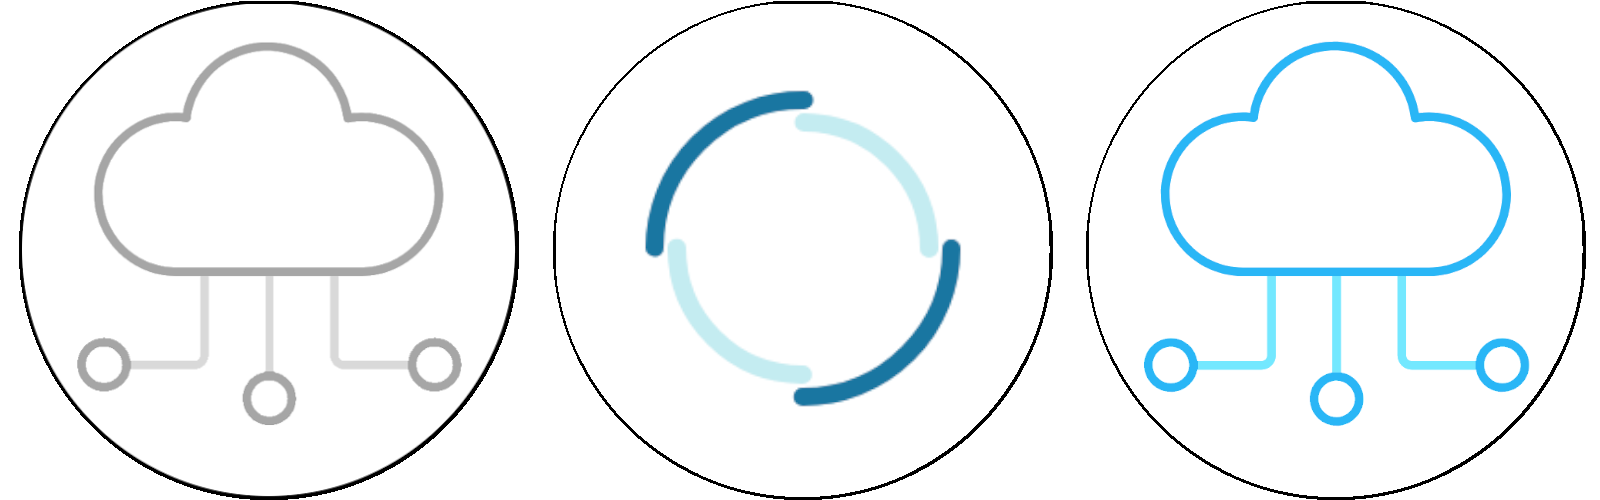
\includegraphics[width=0.6\textwidth]{Connection-Symbols.png}
    \caption{Symbole der Verbindungszustände} 
\end{figure}
\noindent
Neben dem Verbindungszustand wird auch die aktuelle Internetgeschwindigkeit in Form von verschiedenen Symbolen, welche in Figma erstellt wurden, angezeigt.
\\ \ \\
In Abbildung 7.2 sind die Symbole der Internetgeschwindigkeit von keiner Verbindung bis hin zur einer schnellen Internetgeschwindigkeit dargestellt.
\\
\begin{figure}[H]
    \centering
    
\includegraphics[width=0.4\textwidth]{Speed-Symbols.png}
    \caption{Verschiedene Symbole der Internetgeschwindigkeit} 
\end{figure}

\pagebreak

\subsubsection{Design des Zustandes Not Connected}

Der Startzustand, welcher direkt nach dem Öffnen der Desktop-Anwendung angezeigt wird ist der Not Connected-Zustand. In diesem Zustand wird der Hintergrund mit der Farbe Rot angezeigt. Das Textfeld in der Mitte der Anwendung zeigt hierbei immer den aktuellen Zustand, in diesem Fall Not Connected, an. Weiters lassen das ausgegraute Verbindungssymbol in der Mitte, sowie das durchgestrichene Geschwindigkeitssymbol am rechten oberen Rand darauf schließen, dass man aktuell mit keinem Server verbunden ist.
Der im unteren Teil der Desktop-Anwendung befindliche Connect-Button zeigt dem Benutzer mit dem Text Select Server, dass ein Server zum Verbinden ausgewählt werden muss.
\\ \ \\
Mit einem Klick auf den Pfeil, welcher sich auf der rechten Seite des Connect-Buttons befindet, öffnet sich eine DropUp-Liste mit allen zuvor im Menü hinzugefügten Servern. Nachdem man den gewünschten Server ausgewählt hat ändert sich die Farbe des Button auf intensiveres Grün und der Text auf Connect to \textit{Servername}. Hiermit wird dem Benutzer signalisiert, dass nun durch einen Mausklick auf die Mitte des Buttons der Verbindungsaufbau mit dem gewählten Server gestartet werden kann.
\\
\begin{figure}[H]
    \centering
    \setlength{\fboxsep}{1pt}
	\setlength{\fboxrule}{1pt}
	\fbox{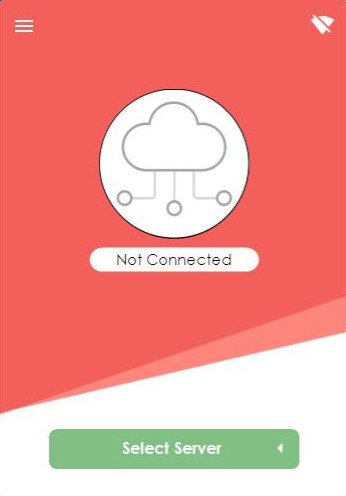
\includegraphics[width=0.4\textwidth]{NotConnected.jpg}}
    \caption{Design der Desktop-Anwendung im Zustand Not Connected} 
\end{figure}

\pagebreak

\subsubsection{Design des Zustandes Connecting}

Startet der Benutzer den Verbindungsaufbau, wechselt die Desktop-Anwendung in den Zustand Connecting. Hier wird der Hintergrund in der Farbe Blau angezeigt. Weiters ändert sich die Farbe des Buttons zu Grau und der Pfeil, welcher die Serverauswahl öffnet, verschwindet. Somit kann in der Zeit des Verbindens kein neuer Server ausgewählt werden. Auch kann nicht auf das Menü-Icon, welches die Einstellungen öffnet, gedrückt werden. Das Textfeld in der Mitte der Anwendung zeigt nun Connecting an und die animierte Ladeanimation deutet darauf hin, dass sich der Treiber mit dem ausgewählten Server verbindet.
\\
\begin{figure}[H]
    \centering
    \setlength{\fboxsep}{1pt}
	\setlength{\fboxrule}{1pt}
	\fbox{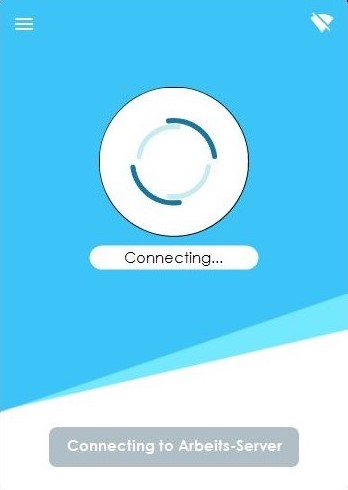
\includegraphics[width=0.4\textwidth]{Connecting.jpg}}
    \caption{Design der Desktop-Anwendung im Zustand Connecting} 
\end{figure}

\subsubsection{Design des Zustandes Connected}

Nach einem erfolgreichen Verbindungsaufbau wechselt die Desktop-Anwendung in den dritten Zustand Connected. In diesem Zustand wird der Hintergrund in der Farbe Grün angezeigt. Das Textfeld in der Mitte der Anwendung sagt nun “Connected to Servername”. Weiters lässt das darüberliegende Verbindungssymbol darauf schließen, dass man mit dem Server verbunden ist. Der Connect-Button hat sich auf die Farbe Rot und der Text auf Disconnect geändert. Das im rechten oberen Eck der Desktop-Anwendung befindliche Internetgeschwindigkeitssymbol hat neben der visuellen Darstellung nun auch eine weitere Funktion. Wenn man mit der Maus über das Symbol fährt erscheint links daneben eine Anzeige, welches dem Benutzer Auskunft über die aktuelle Internetgeschwindigkeit im Format Megabit pro Sekunde sowie den aktuellen Ping im Format Millisekunden gibt.
\\
\begin{figure}[H]
    \centering
    \setlength{\fboxsep}{1pt}
	\setlength{\fboxrule}{1pt}
	\fbox{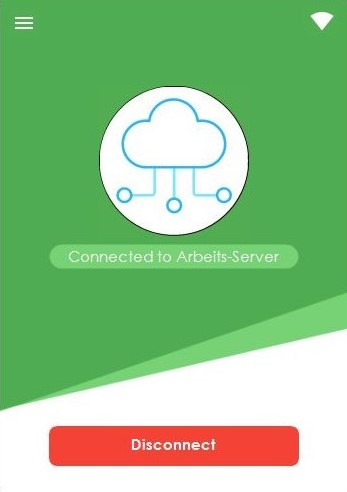
\includegraphics[width=0.4\textwidth]{Connected.jpg}}
    \caption{Design der Desktop-Anwendung im Zustand Conneted} 
\end{figure}

\subsubsection{Design des Fensters}

Viele Komponenten der Desktop-Anwendung wie Buttons und Textfelder haben ein modernes Design mit abgerundeten Ecken. Um eine einheitliche Designsprache zu gewährleisten soll auch das Fenster runde Ecken bekommen. Hierfür muss die Dynamic Link Library Gdi32\footnote[1]{\cite[Vgl.][]{GDI}} von Windows importiert werden. Diese beinhaltet die Methode \mbox{CreateRoundRectRgn()}, mit welchem ein neues Fenster mit angegebener Ellipsengröße für die Ecken erstellt werden kann.

\begin{program}[H]
\begin{CSharpCode}
Region = Region.FromHrgn(CreateRoundRectRgn(0, 0, Width, Height, 10, 10));
\end{CSharpCode}
\caption{Erstellen eines neuen Fensters mit abgerundeten Ecken}
\end{program}

\subsection{Design und Funktionalität des Connect-Buttons}

Der Connect-Button ist einer der wichtigsten Elemente der Desktop-Anwendung. Mithilfe diesem ist es möglich einen Server auszuwählen und sich mit diesem zu verbinden. Nach einem erfolgreichen Verbindungsaufbau kann man mit dem selben Button die Verbindung zum Server wieder trennen. Zusätzlich zur beschriebenen Funktionalität soll das Bedienelement über ein modernes Design mit abgerundeten Ecken verfügen.
\\ \ \\
Möchte man nun einen Button mit genau diesen Anforderungen in die Realität umsetzen, stößt man in WinForms mit den Standard-Windows-Bedienelementen auf drei wesentliche Probleme.
\\
\begin{enumerate}
 \item Der Standard-Button von WinForms ist viereckig und es gibt keine Möglichkeit dies zu ändern.
 \item Der Button soll über ein DropUp-Menü verfügen, welches eine Liste von Servern beinhaltet. Weiters soll man durch einen Mausklick auf diesen einen der Server auswählen können um sich damit zu verbinden. WinForms bietet zwar für solche Fälle eine sogenannte ComboBox an, doch diese hat erstens nur ein DropDown-Menü und zweitens stößt man bei der Benutzung dieser Komponente auf ein weiteres, nun folgendes Problem.
 \item Der Button soll zweigeteilt sein. Das bedeutet dass durch das Klicken auf das Bedienelement einerseits das Verbinden mit einem Server, andererseit aber auch das Öffnen des DropUp-Menüs möglich sein muss. Somit muss je nach Position des Mauszeigers beim Klick auf den Button eine andere Funktionalität verfügbar sein was mit dem Standard-Button ebenfalls nicht umsetzbar ist.
\end{enumerate}
\ \\
Die von uns verwendete Dynamic Link Library MetroSuite bietet zwar einen eigenen sogenannten MetroButton bei welchem man per Einstellung die Kanten abrunden kann, doch die 2 anderen Probleme können auch mit der Benutzung der DLL nicht gelöst werden. Daher können wir die Standard-Windows-Bedienelemente nicht benutzen und müssen einen eigenen Button programmieren.
\\ \ \\
In Abbildung 7.6 sind das gewünschte Design und die Funktionalität des Connect-Buttons dargestellt.
\begin{figure}[H]
    \centering
    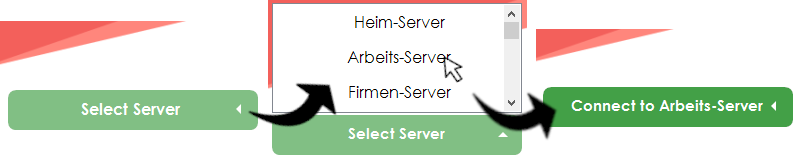
\includegraphics[width=1\textwidth]{connectButton.png}
    \caption{Design und Funktionalität des Connect-Buttons} 
\end{figure}

\subsubsection{Inhalt der Klasse Connect-Button}

Um einen eigenen Button mit unseren Wünschen zu kreieren, haben wir eine eigene Klasse namens ConnectButton, welche von der Standard-Button-Klasse abgeleitet ist, geschrieben. Die Button-Klasse ist Teil des System.Windows.Form-Namespaces, welcher alle User-Interface-Komponenten von Windows beinhaltet. Somit benutzen wir die schon vorhandenen Funktionalitäten eines Windows-Buttons und ergänzen diese mit eigenen zusätzlichen Funktionen und einem neuen Design.
\\ \ \\
Zum Designen des neuen Buttons benutzen wir die Klasse GraphicsPath, welche Teil vom System.Drawing.Drawing2D-Namespace ist. Mithilfe dieser Klasse ist es möglich Formen und Figuren mit der integrierten Grafik-Engine zu erstellen. Hierfür stellt die Klasse eine Reihe an Methoden zur Verfügung, mit welchen man neue Formen zu seiner Figur hinzufügen kann. In unseren Fall wurde die beiden Methoden AddLine() und AddArc() verwendet. Mithilfe dieser konnte die Form eines Buttons mit vier Linien und vier runden Ecken nachgebildet werden.

\begin{program}[H]
\begin{CSharpCode}
GraphicsPath graphPath = new GraphicsPath();
graphPath.AddLine(x1, y1, x2, y2);
\end{CSharpCode}
\caption{Hinzufügen einer Linie zu einer Figur}
\end{program}
\noindent 
Damit die erstellte Figure auch gezeichnet wird, muss noch die OnPaint-Methode der abgeleiteten Klasse Button überschrieben werden. In dieser Methode würde normalerweise der Standard-Windows-Button gezeichnet werden. Da hier aber jetzt unsere eigene Figure gezeichnet werden soll löschen wir das bestehende Design und zeichnen mit der Methode FillPath() die neue Figur.

\begin{program}[H]
\begin{CSharpCode}
protected override void OnPaint(PaintEventArgs paintEvent)
{
    paintEvent.Graphics.FillPath(brush, graphPath);
}
\end{CSharpCode}
\caption{Zeichnen einer Figur}
\end{program}
\noindent 
Wenn man nun den Connect-Button erstellt wird man bemerken, dass dieser vor allem in den Ecken nicht schön rund sondern eher verpixelt von der Grafik-Engine gezeichnet wurde. Um diesem Problem entgegenzuwirken müssen in der OnPaint()-Methode noch einige Einstellungen über die Renderqualität getätigt werden.

\begin{program}[H]
\begin{CSharpCode}
paintEvent.Graphics.InterpolationMode = InterpolationMode.HighQualityBilinear;
paintEvent.Graphics.CompositingQuality = CompositingQuality.HighQuality;
paintEvent.Graphics.PixelOffsetMode = PixelOffsetMode.HighQuality;
paintEvent.Graphics.SmoothingMode = SmoothingMode.AntiAlias;
\end{CSharpCode}
\caption{Beispiel-Code zum Verbessern der Renderqualität}
\end{program}
\noindent 
Mithilfe dieser vier Methoden werden alle wichtigen, für die Zeichen- und Renderqualität verantwortlichen Parameter auf die maximale Qualität gestellt um die bestmögliche Grafik zu erzielen. 
\\ \ \\
Neben einem Text soll auf der rechten Seite des Connect-Buttons auch ein Pfeil angezeigt werden, welcher dem Benutzer zeigt, dass man mit einem Mausklick auf diesen die Drop-Up-Liste öffnen beziehungsweise schließen kann. Dieser Pfeil soll je nachdem ob die Liste gerade geöffnet oder geschlossen ist, nach oben oder nach links zeigen. Hierfür wurden zwei verschiedene Pfeile für die beiden Richtungen in Figma kreiert. Die beiden Grafiken werden mithilfe der Klasse Icon eingelesen und können dann mit der Methode DrawIcon() an einer bestimmten Stelle im Button gezeichnet werden. Wichtig hierbei ist, dass die eingebundenen Icons vom Typ .ico sein müssen! 

\begin{program}[H]
\begin{CSharpCode}
Icon arrow = new Icon("arrow.ico");
paintEvent.Graphics.DrawIcon(arrow , x, y);
\end{CSharpCode}
\caption{Zeichnen eines Icons}
\end{program}
\noindent 
Da der Connect-Button durch das Klicken auf zwei verschiedene Stellen zwei verschiedene Funktionalitäten haben soll muss hier mit der Position des Mauszeigers beim Klick gearbeitet werden. Zuerst wird ein MouseUp-Event definiert, welches beim wieder Loslassen nach dem Drücken der linken Maustaste aktiviert wird. Nun kann mit MousePosition.X die X-Koordinate der aktuellen Position des Mauszeigers abgerufen werden. Mithilfe dieser Koordinate kann man überprüfen ob der Benutzer die Drop-Up-List aufrufen oder den Verbindungsaufbau starten möchte. Falls noch kein Server ausgewählt worden ist, ist der Mausklick zum Verbinden wirkungslos.

\subsubsection{Design und Funktionalität der Drop-Up-Liste}

Die Drop-Up-Liste soll die Möglichkeit bieten einen Server auszuwählen, um sich mit diesem zu verbinden. Hierfür verwenden wir die ListBox von WinForms. Diese Komponente ermöglicht standardmäßig das Hinzufügen von Einträgen, das Auswählen dieser, sowie das Nutzen einer Scrollbar. Zusätzlich dazu wurde auch dieses UI-Element an unserer Wünsche angepasst und um einige Funktionalitäten erweitert. Das Ziel ist, genauso wie beim Connect-Button, das Design zu verbessern. Die Änderungen umfassen das Anpassen der Schriftart/-größe und der Position, sowie das Verhalten beim Auswählen eines Servers durch einen Mausklick auf diesen.
\\ \ \\
Um die gewünschten Änderungen umzusetzen muss nicht wie beim Connect-Button eine eigene Klasse erstellt und die OnPaint()-Methode überschrieben werden. Hierfür gibt es das ListBox-Event DrawItem. Mithilfe von Events und Delegates ist es also möglich eine eigene Methode zu schreiben, mit welcher man die Elemente der ListBox selbst zeichnen kann. Wichtig zu erwähnen ist, dass wenn man diese Methode verwenden möchte, vorher noch die Option DrawMode der ListBox auf OwnerDrawFixed gestellt werden muss!
\\ \ \\
Nun haben wir die Möglichkeit, das Verhalten beim Auswählen eines Listenelementes zu definieren. Hierfür wird mit einem If-Anweisung überprüft ob das Listenelement ausgewählt wurde. Falls das der Fall ist, wird die Schriftart auf Fett geändert und die Schriftfarbe auf Grün.

\begin{program}[H]
\begin{CSharpCode}
if (drawEvent.State == DrawItemState.Selected)
{
    drawEvent = new DrawItemEventArgs(/*Parameter*/);
}
\end{CSharpCode}
\caption{Ändern der Eigenschaften eines ausgewählten Listenelements}
\end{program}
\noindent
Nach dem Definieren aller weiteren Parameter, wie Standard-Schriftart, -farbe und -größe muss das Listenelement noch gezeichnet werden. Hierfür kommt die Methode DrawString() zum Einsatz. Da hier auch Informationen über die Position angegeben werden müssen, kann so auch gleich definiert werden, dass das Element mittig in der ListBox zentriert gezeichnet werden soll.

\begin{program}[H]
\begin{CSharpCode}
drawEvent.Graphics.DrawString(text, font, brush, x, y);
\end{CSharpCode}
\caption{Zeichnen eines Listenelementes}
\end{program}
\noindent
Zum Einstellen des Abstandes zwischen den Listenelementen gibt es die ListBox-Eigenschaft ItemHeight. Mithilfe dieser kann der gewünschte Wert definiert werden. Hierfür muss aber die Option DrawMode der ListBox auf OwnerDrawVariable gestellt werden.

\subsection{Design und Funktionalität des Menüs}
Mit einem Mausklick auf das Icon in der linken oberen Ecke der Desktop-Anwendung gelangt man in das Menü. Hier können wichtige Einstellungen getätigt werden. Das Menü ist in die drei Menüpunkte Mode, Server und Network Devices unterteilt. Jeder der Menüpunkte wird durch ein eigenes, zur Einstellungsmöglichkeit passendes, Icon repräsentiert. Diese wurden in Figma erstellt. Mit einem Klick auf den jeweiligen Unterpunkt kommt man zu deren spezifischen Einstellungen. Um das Menü wieder zu verlassen, muss man auf den Schließen-Button, welcher sich oben links befindet klicken.
\\
\begin{figure}[H]
    \centering
    \setlength{\fboxsep}{1pt}
	\setlength{\fboxrule}{1pt}
	\fbox{\includegraphics[width=0.4\textwidth]{Menü.jpg}}
    \caption{Design des Menüs mit den drei Menüpunkten} 
\end{figure}

\pagebreak
\subsubsection{Design des Menüpunktes Mode}

Bei den Modus-Einstellungen, kann man definieren in welchem Modus der Treiber laufen soll. Man soll zwischen dem Perfomance-basierenden und Kostenbasierenden Modus auswählen können. Da wir uns im Rahmen der Diplomarbeit ausschließlich auf den ersten der beiden Modis konzentrieren dient der Menüpunkt Mode aktuell nur als Beschreibung des Kosten-basierenden Modus. Der ausgegraute Button mit dem Text “Selected” unterhalb der Kurzbeschreibung zeigt dem Benutzer, dass akutell dieser Modus ausgewählt ist. Mit einem Klick Mausklick auf den Pfeil links oben kommt man wieder in die Einstellungsübersicht zurück.
\\
\begin{figure}[H]
    \centering
    \setlength{\fboxsep}{1pt}
	\setlength{\fboxrule}{1pt}
	\fbox{\includegraphics[width=0.4\textwidth]{MenüMode.jpg}}
    \caption{Design des Menüpunktes Mode} 
\end{figure}

\subsubsection{Design des Menüpunktes Server}

Bei den Server-Einstellungen hat der Benutzer die Möglichkeit, Server zu verwalten.
Im oberen Bereich mit der Aufschrift “Add Server” kann man einen neuen Server hinzuzufügen. Hier muss der Name, welcher frei wählbar ist, die IP-Adresse und der Post des Servers eingetragen werden. Mit einem Klick auf “Add” wird der Server in die darunterliegende Liste hinzugefügt. Im unteren Bereich namens “Server List” werden alle gespeicherten Server angezeigt. Mit einem Mausklick auf einen Server wird die Schriftart Fett und die Schriftfarbe Blau angezeigt. Somit wurde der Server als Default-Server festgelegt. Mit dem Löschen-Button, welcher sich unterhalb der Liste befindet, kann ein ausgewählter Server wieder von der Liste entfernt werden.
\\
\begin{figure}[H]
    \centering
    \setlength{\fboxsep}{1pt}
	\setlength{\fboxrule}{1pt}
	\fbox{\includegraphics[width=0.4\textwidth]{MenüServer.jpg}}
    \caption{Design des Menüpunktes Server} 
\end{figure}
\noindent
WinForms bietet keine Möglichkeit, das Verhalten bei der Auswahl eines Listenelementes zu ändern. Daher kamen genauso wie bei der Drop-Up-Liste des ConnectButtons Event, Delegates und die Methode DrawItem() zum Einsatz um die Listenelement manuell zu zeichnen. Nur so konnte das Ändern der Schrifteigenschaften möglich gemacht werden.

\subsubsection{Speichern der Serverliste}
Da zur Serverliste hinzugefügte Server auch nach dem Schließen und einem erneuten Öffnen der Desktop-Anwendung noch zur Verfügung stehen sollen, müssen wichtige Einstellungen wie die Serverliste gespeichert werden. Hierfür benutzen wird den System.Text.Json-Namespace welcher es ermöglicht, Objekte ins JSON-Format zu serialisieren und vom JSON-Format wieder in Objekte zu deserialisieren.
\\ \ \\
Zur Speicherung relevante ist eine Liste mit allen Servern, welche wiederum aus den drei Attributen Name, IP-Adresse und Port bestehen. Um diese Daten einfach zu speichern und später wieder auslesen zu können haben wir eine Klasse namens ServerObject erstellt, welche die drei Attribute beinhaltet. Eine zweite Klasse ServerSettings speichert diese Server-Objekte in einer Liste.

\begin{program}[H]
\begin{CSharpCode}
public class ServerObject
{
    public string name { get; set; }
    public string ip { get; set; }
    public int port { get; set; }
}
\end{CSharpCode}
\caption{Aufbau der Klasse ServerObject}
\end{program}
\noindent
Wird nun ein neuer Server in der Desktop-Anwendung hinzugefügt, wird ein neues Server-Objekt erstellt und in die Serverliste hinzugefügt. Sollte ein bestehender Server gelöscht werden, wird das Server-Objekt wieder aus der Liste entfernt.
\\ \ \\
Schließt der Benutzer nun die Desktop-Anwendung werden mögliche Änderungen in der Serverliste gespeichert werden. Hierfür kommt der im System.Text.Json-Namespace enthaltene JsonSerializer zum Einsatz. Dieser serialisiert ein ServerSettings-Objekt, welches die Liste mit allen Servern-Objekten beinhaltet, zu einem JSON-Text. Dieser wird dann in eine Datei names serverSettings.json im selben Verzeichnis wo auch die .exe-Datei liegt gespeichert.

\begin{program}[H]
\begin{CSharpCode}
public class ServerObject
string settings = JsonSerializer.Serialize(serverSettings);
\end{CSharpCode}
\caption{Serialisieren des serverSettings-Objektes}
\end{program}
\noindent
Startet der Benutzer die Desktop-Anwendung, werden alle gespeicherten Einstellungen wieder geladen. Hierfür wird der gespeicherte JSON-Text aus der Datei ausgelesen und mit dem JsonSerializer deserialisiert.

\begin{program}[H]
\begin{CSharpCode}
serverSettings = JsonSerializer.Deserialize<ServerSettings>(settings);
\end{CSharpCode}
\caption{Deserialisieren des eingelesenen JSON-Textes}
\end{program}
\noindent
Nachdem das einlesen erfolgreich abgeschlossen wurde, werden die Serverliste im Menü sowie die Drop-Up-List vom Connect-Button mit den gespeicherten Einstellungen befüllt.

\subsubsection{Design des Menüpunktes Network Devices}

Bei den Netzwerkadapter-Einstellungen kann der Benutzer die Netzwerkadapter verwalten. Hierfür werden im Bereich mit der Aufschrift \grqq Network Devices List\grqq{} alle verfügbaren Netzwerkadapter aufgelistet. Durch einen Mausklick auf einen Listeneintrag wird die Schriftart Fett und die Schriftfarbe Blau. Somit wurde der Netzwerkadapter ausgewählt und wird nun vom Treiber verwendet. Mit einem erneuten Klick kann dieser auch wieder abgewählt werden. Für die Erweiterung des Kosten-basierenden Modus, würde noch die Angabe der Kosten pro Megabyte hinzukommen.
\\
\begin{figure}[H]
    \centering
    \setlength{\fboxsep}{1pt}
	\setlength{\fboxrule}{1pt}
	\fbox{\includegraphics[width=0.4\textwidth]{MenüNetworkDevices.jpg}}
    \caption{Design des Menüpunktes Network Devices} 
\end{figure}

\subsubsection{Einlesen der Netzwerkadapter}

Um die Netzwerkadapter auswählen zu können, müssen diese beim Start der Desktop-Anwendung eingelesen werden. Hierfür muss die Klasse Win32\_NetworkAdapterConfiguration instanziiert werden. Diese beinhaltet alle Attribute und Methoden der Netzwerkadapter. Das Attribut Description liefert uns den Namen des Netzwerkadapters, welchen wir in die Network-Devices-Liste speichern können. Mithilfe der Variable ipEnabled werden nur aktivierten Netzwerkadapter angezeigt.

\begin{program}[H]
\begin{CSharpCode}
if ((bool)managementObject["ipEnabled"])
{
    netDevices.Add(managementObject["Description"].ToString());
}
\end{CSharpCode}
\caption{Einlesen der Namen der aktiven Netzwerkadapter}
\end{program}
\noindent
Da die Namen der Netzwerkadapter oft zu breit für die Darstellung in der ListBox sind, muss gegebenenfalls eine horizontale Scrollbar angezeigt werden. Hierfür wird nach dem Einfügen der Adapter mithilfe der MeasureString()-Methode die Länge der Namen ermittelt.

%Setzen der Schriftgröße für die Code-Beispiele von Martin
\lstset{basicstyle=\footnotesize}

\pagebreak

\section{Desktop-Anwendung in der Notification Area}
Wir haben unsere Windows Desktop-Anwendung zum Steuern des Multi-Wan Bonding fähigen Treibers als Notification Area Programm entwickelt. Dabei war es uns sehr wichtig, dass der Benutzer einmal auf das Symbol klicken kann, damit wird ihm die wie im Kapitel 7.1 beschriebene Benutzeroberfläche angezeigt. Wenn er jetzt nochmals darauf oder woanders hin drückt, soll die Benutzeroberfläche verborgen werden
\\\\
Um eine Notification Area Anwendung zu implementieren, haben wir eine C\# Klasse entwickelt, diese Klasse ist von \textbf{ApplicationContext} abgeleitet. In dieser Klasse wird ein \textbf{NotifyIcon} angelegt. Dieses \textbf{NotifyIcon} benötigt ein Symbol, mit diesem wird dann die Anwendung in der Notfication Area abgelegt, einen Text der erscheint, sobald sich die Maus über dem Symbol befindet, in unserem Fall "NetShare". Weiters hat das Symbol einen Button zum Schließen der Anwendung, sobald das Symbol mit der rechten Maustaste angeklickt wurde. Wenn dieser Knopf gedrückt wird beendet sich die Windows Desktop-Anwendung und auch der Multi-Wan Bonding fähige Treiber.
\begin{figure}[H]
    \centering
    
\includegraphics[width=5cm, height=5cm, keepaspectratio]{NAIcon.png}
    \caption[NotificationArea]{Netshare Symbol in der Notification Area} 
\end{figure}
\noindent

\newpage
\subsection{Relative Positionierung der grafischen Oberfläche}
Die Grafische Oberfläche der Windows Desktop-Anwendung soll sich immer an der richtigen Stelle relativ zur Taskleiste positionieren. Mithilfe von \textbf{Screen.PrimaryScreen.Bounds} und \textbf{Screen.PrimaryScreen.WorkingArea} finden wir heraus wo sich die Taskleiste befindet. Mit diesem Wissen setzen wir dann die relative Positionierung der grafischen Oberfläche. \textbf{Screen.PrimaryScreen.Bounds} gibt einem die gesamte Größe des Bildschirms an, \textbf{Screen.PrimaryScreen.WorkingArea} gibt einem die Größe an in der z.B. auch Webbrowser geöffnet sind, also ohne der  Taskleiste. Im Codebeispiel sieht man wie dies funktioniert, wenn sich die Taskleiste am unteren Rand befindet.
\begin{program}[H]
\caption{Taskleiste unten}
\begin{CSharpCode}
if((Screen.PrimaryScreen.Bounds.Height - Screen.PrimaryScreen.WorkingArea.Height)>0)
{
    this.Location = new Point(Screen.PrimaryScreen.WorkingArea.X + 
      Screen.PrimaryScreen.WorkingArea.Width - Width - 10, 
      Screen.PrimaryScreen.WorkingArea.Y + Screen.PrimaryScreen.WorkingArea.Height 
      - Height);
}
\end{CSharpCode}
\end{program}
\noindent

\section{Kommunikation zwischen dem Multi-Wan Bonding fähigen Treiber und der Windows Desktop-Anwendung}
Die Windows-Desktop Anwendung muss für das Steuern des Multi-Wan Bonding fähigen Treibers mit diesem Kommunizieren. Wir haben uns als Interprozesskommunikationsart für Sockets entschieden, da wir dies für am einfachsten angesehen haben, weil man sich nicht um die Synchronisation kümmern muss. Der Multi-Wan Bonding fähige Treiber erstellt einen Server der auf "localhost" \ auf dem Port 5260 lauscht und wartet bis sich ein Client mit ihm verbindet. Die Windows Desktop-Anwendung erstellt für jeden Steuerungsbefehl an den Multi-Wan Bonding fähigen Treiber einen Client, der sich zum Server verbindet und dann ein JSON Objekt mit dem jeweiligen Befehl zum Server sendet. Sobald die Windows Desktop-Anwendung die erwartete Antwort bekommen hat, wird die Verbindung zum Multi-Wan Bonding fähigen Treiber geschlossen.

\newpage
\subsection{JSON Object}
\subsubsection{Anfrage (Request)}
Wenn die Windows Desktop-Anwendung eine Anfrage an den Multi-Wan Bonding fähigen Treiber sendet, hat das JSON Objekt folgende Struktur.
\begin{program}[H]
\caption{JSON Anfrage}
\begin{GenericCode}
    {
        "type" :  "",
        "on" :  "",
        "data" : {} 
    }
\end{GenericCode}
\end{program}
\noindent
Bei dem Schlüssel \textbf{type} wird vom Multi-Wan Bonding fähigen Treiber \textbf{Get} oder \textbf{Put} erwartet. Mit \textbf{Get} kann die Windows-Desktop Anwendung die derzeitige Konfiguration oder die Download und Upload Geschwindigkeiten des Multi-Wan Bonding fähigen Treibers anfordern. Mithilfe von \textbf{Put} werden Einstellungen hinzugefügt oder geändert. 
\\\\
Bei dem Schlüssel \textbf{on} gibt es die Werte \textbf{driver.state}, \textbf{deamon.state}, \textbf{connection.state}, \textbf{config} und \textbf{statistics}. Mit \textbf{driver.state} verbindet sich der Multi-Wan Bonding fähige Treiber mit dem Multi-Wan Bonding fähigen Server oder bricht die Verbindung ab. Mithilfe von \textbf{deamon.state} kann man den Multi-Wan Bonding fähigen Treiber beenden. Mit \textbf{connection.state} kann man die Verbindung zwischen dem Server und dem Client von der Server Seite aus beenden und mit \textbf{config} kann man die derzeitigen Konfigurationen anpassen oder anfordern. Mit dem Wert \textbf{statistics} erhält man die Download und Upload Geschwindingkeiten.
\\\\
Bei dem Schlüssel \textbf{data} wird der Wert \textbf{state} erwartet, falls bei dem Schlüssel on der Wert \textbf{driver.state}, \textbf{deamon.state} oder \textbf{connection.state} ist. Wenn der vorherige Schlüssel \textbf{config} ist, wird bei \textbf{data} entweder \textbf{logLevel}, \textbf{serverIp}, \textbf{adapterIp}, \textbf{adapterSubnetBits}, \textbf{names} oder nichts, falls man die gesamte Konfiguration erhalten will, dies ist aber nur möglich, wenn bei dem Schlüssel \textbf{type} der Wert \textbf{Get} ist. Wenn beim Schlüssel \textbf{on} \textbf{statistics} steht, ist wird in \textbf{data} ebenfalls nichts erwartet. 


\subsubsection{Antwort (Response)}
Wenn der Multi-Wan Bonding Server eine Antwort an die Windows-Desktop Anwendung sendet, ist das JSON Objekt folgendermaßen aufgebaut.
\begin{program}[H]
\caption{JSON Antwort}
\begin{GenericCode}
    {
        "type" :  "",
        "data" : {}
    }
\end{GenericCode}
\end{program}
\newpage
\noindent
Bei dem Schlüssel \textbf{type} gibt es zwei mögliche Werte entweder \textbf{Response} oder \textbf{Update}. Mit \textbf{Response} wird mitgeteilt das eine Anfrage fertig abgearbeitet ist. Mithilfe von \textbf{Update} wird ausgedrückt, dass der Multi-Wan Bonding fähige Treiber etwas geändert hat.
\\\\
Beim Schlüssel \textbf{data} steht, falls ein Fehler aufgetreten ist \textbf{error}, ansonsten \textbf{state}, der angeforderte Konfigurationswert, alle konfigurierten Werte mit dem jeweiligen Werten drinnen oder \textbf{down} mit einem Wert und \textbf{up} mit einem Wert.  


\subsection{Verbinden des Multi-Wan Bonding fähigen Treibers mit einem Multi-Wan Bonding fähigen Server}
Um mithilfe des Multi-Wan Bonding fähigen Treibers die Verbindung zum Multi-Wan Bonding fähigen Server herzustellen, wird eine Anfrage von der Windows-Desktop Anwendung gesendet. Diese Anfrage ist folgendermaßen aufgebaut:
\begin{program}[H]
\caption{JSON Anfrage verbinden}
\begin{GenericCode}
    {
        "type" :  "Put",
        "on" :  "driver.state",
        "data" : {"state" : "running"} 
    }    
\end{GenericCode}
\end{program}
\noindent
Daraufhin checkt der Multi-Wan Bonding fähige Treiber ob dieser schon mit dem Multi-Wan Bonding fähigen Server verbunden ist, falls dies der Fall ist, wird diese Antwort gesendet:
\begin{program}[H]
\caption{JSON Antwort verbinden running}
\begin{GenericCode}
    {
        "type" :  "Response",
        "data" : {"state" : "running"} 
    }    
\end{GenericCode}
\end{program}
\noindent
Falls der Multi-Wan Bonding fähige Treiber sich gerade mit dem Multi-Wan Bonding fähigen Server verbindet oder noch keine Verbindung aufgebaut ist, wird beim Schlüssel \textbf{state} der Wert \textbf{startup} eingetragen und als Antwort gesendet. Nachdem die Verbindung erfolgreich aufgebaut wurde, wird das JSON Objekt von vorher gesendet. Wenn die Verbindung nicht aufgebaut werden kann, bekommt man folgende Antwort:
\begin{program}[H]
\caption{JSON Antwort verbinden crashed}
\begin{GenericCode}
    {
        "type" :  "Response",
        "data" : {"state" : "crashed"} 
    }    
\end{GenericCode}
\end{program}
\newpage
\noindent
Nachdem man diese Antwort bekommen hat, versucht die Windows Desktop-Anwendung es noch zweimal, indem sie wieder die Anfrage an den Multi-Wan Bonding fähigen Treiber sendet. Falls bei den zwei weiteren Anfragen auch nur der Wert \textbf{crashed} bei dem Schlüssel \textbf{state} zurückkommt, wird dem Benutzer eine Fehlermeldung angezeigt, die Ihn dazu auffordert den Multi-Wan Bonding fähigen Treiber neu zu starten.


\subsection{Verbindung zu einem Multi-Wan Server trennen}
Um die Verbindung zwischen dem Multi-Wan Bonding fähigen Treiber und dem Multi-Wan Bonding fähigen Server zu trennen, wird eine Anfrage von der Windows Desktop-Anwendung gesendet. Diese Anfrage ist folgendermaßen aufgebaut:
\begin{program}[H]
\caption{JSON Anfrage Verbindung trennen}
\begin{GenericCode}
    {
        "type" :  "Put",
        "on" :  "driver.state",
        "data" : {"state" : "stopped"} 
    }     
\end{GenericCode}
\end{program}
\noindent
Der Multi-Wan Bonding fähige Treiber sendet als Antwort seinen derzeitigen Status, diese Antwort wird so gesendet:
\begin{program}[H]
\caption{JSON Antwort Verbindung trennen}
\begin{GenericCode}
    {
        "type" :  "Response",
        "data" : {"state" : ""} 
    }    
\end{GenericCode}
\end{program}
\noindent
Wobei bei dem Schlüssel \textbf{state} entweder der Wert \textbf{startup}, \textbf{running} oder \textbf{stopped} steht. Falls der Multi-Wan Bonding fähige Treiber als Status nicht \textbf{stopped} hat, bricht der Multi-Wan Bonding fähige Treiber die Verbindung zum Multi-Wan Bonding fähigen Server ab und sendet die Antwort an die Windows Desktop-Anwendung die als \textbf{state} \textbf{stopped} hat.


\subsection{Multi-Wan Bonding fähigen Treiber beenden}
Um den Multi-Wan Bonding fähigen Treiber zu beenden, wird eine Anfrage von der Windows Desktop-Anwendung gesendet. Diese Anfrage ist folgendermaßen aufgebaut:
\begin{program}[H]
\caption{JSON Anfrage Treiber beenden}
\begin{GenericCode}
    {
        "type" :  "Put",
        "on" :  "deamon.state",
        "data" : {"state" : "stopped"} 
    }     
\end{GenericCode}
\end{program}
\newpage
\noindent
Der Multi-Wan Bonding fähige Treiber sendet im Sekundentakt eine Antwort in dieser steht, was der Multi-Wan Bonding fähige Treiber gerade macht. Die Antwort wird mit diesem Aufbau gesendet:
\begin{program}[H]
\caption{JSON Antwort Treiber beenden}
\begin{GenericCode}
    {
        "type" :  "Update",
        "data" : {"state" : ""} 
    }    
\end{GenericCode}
\end{program}
\noindent
Bei dem Schlüssel \textbf{state} steht als Wert entweder \textbf{worker.startup}, \textbf{worker.running} oder \textbf{worker.stopped}. Solange sich der Multi-Wan Bonding fähige Treiber im Status \textbf{startup} befindet, passiert nichts außer, dass die Antwort mit \textbf{worker.startup} sekündlich gesendet wird. Sobald der Status \textbf{running} ist, wird die Antwort mit \textbf{worker.running} gesendet und die Anwendung bekommt den Befehl sich zu schließen. Wenn dies geschehen ist, wird die Antwort mit \textbf{worker.stopped} gesendet. Zusätzlich dazu wird noch eine Antwort gesendet die als \textbf{type} \textbf{Response} hat und bei \textbf{state} den Wert \textbf{stopped} hat.


\subsection{Konfiguration des Multi-Wan Bonding fähigen Treibers ändern}
Um die Einstellungen von dem Multi-Wan Bonding fähigen Treiber zu ändern, wird von der Windows Desktop-Anwendung eine Anfrage gesendet, die folgendermaßen aufgebaut ist:
\begin{program}[H]
\caption{JSON Anfrage Konfiguration ändern}
\begin{GenericCode}
    {
        "type" :  "Put",
        "on" :  "config",
        "data" : {} 
    }     
\end{GenericCode}
\end{program}
\noindent
Bei dem Schlüssel \textbf{data} wird das zu konfigurierende Schlüssel Wert Paar eingetragen. Der Multi-Wan Bonding fähige Treiber sendet als Antwort folgendes JSON-Objekt:
\begin{program}[H]
\caption{JSON Antwort Konfiguration ändern}
\begin{GenericCode}
    {
        "type" :  "Response",
        "data" : {} 
    }    
\end{GenericCode}
\end{program}
\noindent
In \textbf{data} steht das geänderte Schlüssel Wert Paar. Die einzige Änderung die der Multi-Wan Bonding fähige Treiber sofort übernimmt, ist eine Änderung beim \textbf{logLevel}. Jede andere Änderung wird erst verwendet nachdem die Verbindung zum Multi-Wan Bonding fähigen Server getrennt wurde und sich neu mit diesem Verbunden wurde.


\subsection{Konfiguration des Multi-Wan Bonding fähigen Treibers anfordern}
\subsubsection{Gesamte Konfiguration}
Um die gesamte Konfiguration des Multi-Wan Bonding fähigen Treibers zu bekommen, wird von der Windows Desktop-Anwendung eine Anfrage gesendet, die folgendermaßen aufgebaut ist:
\begin{program}[H]
\caption{JSON Anfrage Gesamte Konfiguration anfordern}
\begin{GenericCode}
    {
        "type" :  "Get",
        "on" :  "config",
        "data" : {} 
    }     
\end{GenericCode}
\end{program}
\noindent
Wenn diese Anfrage gesendet wird, antwortet der Multi-Wan Bonding fähige Treiber folgendermaßen:
\begin{program}[H]
\caption{JSON Antwort Gesamte Konfiguration anfordern}
\begin{GenericCode}
    {
        "type" :  "Response",
        "data" : {
                    "logLevel" : "",
                    "serverIp" : "",
                    "serverPort" : "",
                    "adapterIp" : "",
                    "adapterSubnetBits" : "",
                    "names" : []
        } 
    }    
\end{GenericCode}
\end{program}
\noindent
Bei jedem Schlüssel Wert Paar in \textbf{data} wird noch der eingestellte Wert eingetragen.


\subsubsection{Einzelne Einstellungen}
Um nur eine einzelne Konfiguration vom Multi-Wan Bonding fähigen Treiber zu bekommen, wird eine Anfrage von der Windows Desktop-Anwendung gesendet, die folgendermaßen aufgebaut ist:
\begin{program}[H]
\caption{JSON Anfrage einzelne Konfiguration anfordern}
\begin{GenericCode}
    {
        "type" :  "Get",
        "on" :  "config",
        "data" : {} 
    }     
\end{GenericCode}
\end{program}
\noindent
In dem Feld \textbf{data} steht ein Schlüssel Wert Paar als Schlüssel steht die gewünschte Option und als Wert eine Leere Zeichenkette. Der Multi-Wan Bonding fähige Treiber sendet eine Antwort die folgendermaßen Aufgebaut ist: 
\begin{program}[H]
\caption{JSON Antwort einzelne Konfiguration anfordern}
\begin{GenericCode}
    {
        "type" :  "Response",
        "data" : {} 
    }    
\end{GenericCode}
\end{program}
\noindent
In \textbf{data} steht das angeforderte Schlüssel Wert Paar.

\subsection{Upload und Download Geschwindigkeit anfordern}
Um in der Windows Desktop-Anwendung den Upload und den Download Speed anzeigen zu können, wird eine Anfrage an den Multi-Wan Bonding fähigen Treiber gesendet, diese Anfrage ist folgendermaßen aufgebaut:
\begin{program}[H]
\caption{JSON Anfrage Upload Download}
\begin{GenericCode}
    {
        "type" :  "Get",
        "on" :  "statistics",
        "data" : {} 
    }     
\end{GenericCode}
\end{program}
\noindent
Der Multi-Wan Bonding fähige Treiber sendet daraufhin jede Sekunde eine Antwort mit der Upload und Download Geschwindigkeit, diese werden kontinuierlich berechnet. Die Antwort ist folgendermaßen aufgebaut:
\begin{program}[H]
\caption{JSON Antwort Upload Download}
\begin{GenericCode}
    {
        "type" :  "Response",
        "data" : {
                    "down" : "",
                    "up" : ""
        } 
    }    
\end{GenericCode}
\end{program}
\noindent
Die Anfrage an den Mult-Wan Bonding fähigen Treiber wird automatisch gesendet, sobald dieser mit einem Multi-Wan Bonding fähigen Server verbunden ist. 

%Setzen der Schriftgröße für die Code-Beispiele für Manuel
\lstset{basicstyle=\normalsize}

\pagebreak

\section{Windows-Service zur Crash-Recovery des Treibers}

Ein Windows-Service, zu deutsch Windows-Systemdienst, ist ein Programm welches als Dienst im Hintergrund einer Windows-Sitzung läuft\footnote[1]{\cite[Vgl.][]{WindowsService}}. Somit eignet sich ein Windows-Service perfekt für unseren Treiber, welcher immer im Hintergrund laufen, aber den Benutzer nicht stören soll. Weiters soll dieser, bei einem möglichen Absturz, automatisch vom Service neu gestartet werden.

\subsection{Starten des Treibers}

Beim Starten unseres Treibers in Form einer .exe-Datei muss bedacht werden, dass seit der Windows Version Vista ein Windows-Service nicht mehr mit dem Desktop interagieren kann. Das bedeutet, dass der Systemdienst keine Programme mit grafischer Oberfläche starten kann. Da unser Treiber keine grafischen Elemente besitzt kann dieser mit der Angabe von zusätzlichen Parametern gestartet werden.
Mit dem Kofigurieren der Parameter CreateNoWindow und UseShellExecute weiß der Windows-Service, dass keine grafische Oberfläche sowie Shell vom Treiber benutzt wird.

\begin{program}[H]
\begin{CSharpCode}
ProcessStartInfo info = new ProcessStartInfo("netshare.exe");

info.UseShellExecute = false;
info.CreateNoWindow = true;
info.ErrorDialog = false;
info.WindowStyle = ProcessWindowStyle.Hidden;

Process process = Process.Start(info);
\end{CSharpCode}
\caption{Starten des Treibers mit Windows-Service}
\end{program}

\subsection{Crash-Recovery}

Damit sichergestellt werden kann, dass der Treiber immer verfügbar ist, muss im Windows-Service eine Crash-Recovery eingebaut werden. Diese überprüft ob das Programm noch läuft und startet gegebenenfalls den Treiber neu. Das laufende Programm kann mithilfe von \mbox{Process.GetProcessesByName("netshare.exe")} gefunden und somit überprüft werden.
\chapter{Funktionstests für Multi-Wan Bonding}
\label{cha:Funktionstests für Multi-Wan Bonding}

\section{Testaufbau}
Beim Testen unseres Multi-Wan Bonding Prototyps haben wir die folgenden Tests durchgeführt. 

\subsection{Internetverbindung}
Um zu überprüfen, ob wir uns mithilfe unseres Prototyps eine Verbindung mit dem Internet aufbauen zu können, haben wir nur eine Internetanbindung verwendet und versucht google aufzurufen. Als dieses funktioniert hat, haben wir das selbe mit zwei Internetanbindungen versucht.

\subsection{Bündelung}
Um zu untersuchen wie gut es möglich ist Internetanbindungen zu bündeln haben wir einen Performancetest gemacht. Dabei haben wir uns die Downloadgeschwindigkeit, die Uploadgeschwindigkeit und die Latzzeit von unserem Prototyp mit zwei Internetanbindungen angesehen. Diese Werte wurden verglichen mit denen die wir bekommen haben als wir dasselbe ohne unseren Prototyp getestet haben. 

\subsection{Stabilität}
Um die Stabilität zu testen haben wir unseren Prototyp mit zwei Internetanbindung verwendet, und dann die Verbindung zu einer getrennt. Dabei haben wir untersucht ob unsere Internetverbindung abbricht und ob wir Pakete verlieren. 

\section{Ergebnisse der Testdurchführung}
Beim Testen unseres Prototyps sind wir darauf gestoßen, dass es möglich ist mit zwei Internetanbindungen sich mit dem Internet zu verbinden. Beim Performancetest sind wir bei der Downloadgeschwindigkeit auf ca. 60 \% beider Internetanbindung gekommen. Die Uploadgeschwindigkeit war besser, hier haben wir 85 \% der Leistung beider Internetanbindungen bekommen. Die Latzzeit wurde um 2 ms schlechter als bei einer Internetanbindung ohne unseren Prototyp. Unser Prototyp ermöglicht eine unterbrechungsfreihe Internetverbindung auch wenn eine Internetanbindung ausfällt, dies passiert auch ohne Paketverlust.
\chapter{Fazit}
\label{cha:Fazit}


%%%----------------------------------------------------------
%Ausgabe der automatischen Zusatzdaten: Glossar, Index, Literaturverzeichnis
%\clearpage
%\printglossaries

\clearpage
\chapter*{Index}
\addcontentsline{toc}{chapter}{Index}
\printindex[allgemein]

\printindex

\printindex[name]

\printindex[title]


%Literaturverzeichnis
\clearpage
\addcontentsline{toc}{chapter}{\bibname}

\printbibliography

%%%----------------------------------------------------------

%%%Messbox zur Druckkontrolle
%\chapter*{Messbox zur Druckkontrolle}



\begin{center}
{\Large --- Druckgröße kontrollieren! ---}

\bigskip

\Messbox{100}{50} % Angabe der Breite/Hoehe in mm

\bigskip

{\Large --- Diese Seite nach dem Druck entfernen! ---}

\end{center}



\end{document}